% Options for packages loaded elsewhere
\PassOptionsToPackage{unicode}{hyperref}
\PassOptionsToPackage{hyphens}{url}
%
\documentclass[
]{article}
\usepackage{amsmath,amssymb}
\usepackage{iftex}
\ifPDFTeX
  \usepackage[T1]{fontenc}
  \usepackage[utf8]{inputenc}
  \usepackage{textcomp} % provide euro and other symbols
\else % if luatex or xetex
  \usepackage{unicode-math} % this also loads fontspec
  \defaultfontfeatures{Scale=MatchLowercase}
  \defaultfontfeatures[\rmfamily]{Ligatures=TeX,Scale=1}
\fi
\usepackage{lmodern}
\ifPDFTeX\else
  % xetex/luatex font selection
\fi
% Use upquote if available, for straight quotes in verbatim environments
\IfFileExists{upquote.sty}{\usepackage{upquote}}{}
\IfFileExists{microtype.sty}{% use microtype if available
  \usepackage[]{microtype}
  \UseMicrotypeSet[protrusion]{basicmath} % disable protrusion for tt fonts
}{}
\makeatletter
\@ifundefined{KOMAClassName}{% if non-KOMA class
  \IfFileExists{parskip.sty}{%
    \usepackage{parskip}
  }{% else
    \setlength{\parindent}{0pt}
    \setlength{\parskip}{6pt plus 2pt minus 1pt}}
}{% if KOMA class
  \KOMAoptions{parskip=half}}
\makeatother
\usepackage{xcolor}
\usepackage[margin=1in]{geometry}
\usepackage{graphicx}
\makeatletter
\def\maxwidth{\ifdim\Gin@nat@width>\linewidth\linewidth\else\Gin@nat@width\fi}
\def\maxheight{\ifdim\Gin@nat@height>\textheight\textheight\else\Gin@nat@height\fi}
\makeatother
% Scale images if necessary, so that they will not overflow the page
% margins by default, and it is still possible to overwrite the defaults
% using explicit options in \includegraphics[width, height, ...]{}
\setkeys{Gin}{width=\maxwidth,height=\maxheight,keepaspectratio}
% Set default figure placement to htbp
\makeatletter
\def\fps@figure{htbp}
\makeatother
\setlength{\emergencystretch}{3em} % prevent overfull lines
\providecommand{\tightlist}{%
  \setlength{\itemsep}{0pt}\setlength{\parskip}{0pt}}
\setcounter{secnumdepth}{-\maxdimen} % remove section numbering
\usepackage{caption}
\usepackage{fancyhdr}
\pagestyle{fancy}
\fancyhead{} % clear all header fields
\fancyhead[C]{\nouppercase{\leftmark}}
\fancyfoot{}
\fancyfoot[C]{\thepage}
\usepackage{float}
\usepackage{threeparttable}
\usepackage{titling}
\pretitle{\begin{center}\LARGE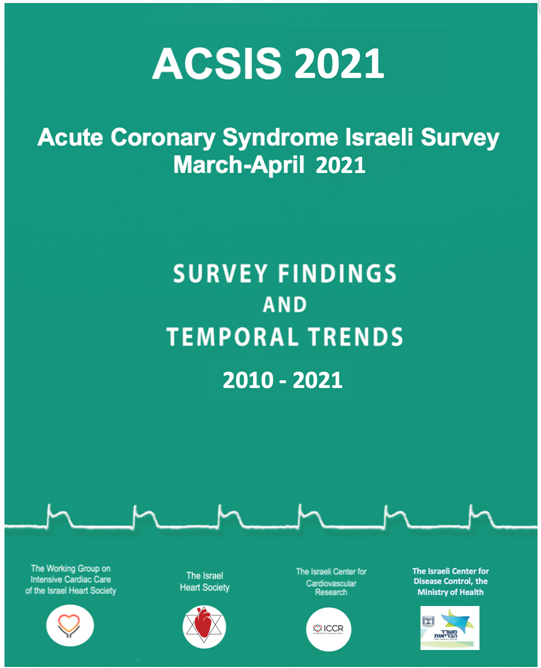
\includegraphics[width=18cm,height=20.5cm,keepaspectratio]{cover_21.png}\\[\bigskipamount]}
\posttitle{\end{center}}
\usepackage{booktabs}
\usepackage{longtable}
\usepackage{array}
\usepackage{multirow}
\usepackage{wrapfig}
\usepackage{float}
\usepackage{colortbl}
\usepackage{pdflscape}
\usepackage{tabu}
\usepackage{threeparttable}
\usepackage{threeparttablex}
\usepackage[normalem]{ulem}
\usepackage{makecell}
\usepackage{xcolor}
\ifLuaTeX
  \usepackage{selnolig}  % disable illegal ligatures
\fi
\usepackage{bookmark}
\IfFileExists{xurl.sty}{\usepackage{xurl}}{} % add URL line breaks if available
\urlstyle{same}
\hypersetup{
  pdftitle={Booklet ACSIS 2024},
  hidelinks,
  pdfcreator={LaTeX via pandoc}}

\title{Booklet ACSIS 2024}
\author{}
\date{\vspace{-2.5em}September 2024}

\begin{document}
\maketitle

{
\setcounter{tocdepth}{2}
\tableofcontents
}
\captionsetup[table]{labelformat=empty}

\pagebreak

\section{Introduction}\label{introduction}

We are proud to present you with the ACSIS 2024 survey results. This
survey, is a biennial tradition since it was launched in 1992 by
Prof.~Shlomo Behar.

The ACSIS survey provides a state-of-the-art representation of the
characteristics, management, and outcome of patients presenting with an
acute coronary syndrome (ACS) in Israel. This survey is a source of
pride for the Israeli cardiology community.

ACSIS 2024 was carried out during March-April 2024 by the Israeli
working group on Acute Cardiac Care of the Israel Heart Society, and the
Israeli Center for Cardiovascular Research (ICCR) in cooperation with
the Israeli Center for Disease Control (ICDC) and Israel Society of
Intensive Care Nursing.

During this 2-month period, detailed data was collected in all intensive
cardiac care units (ICCU) and cardiology wards in all public hospitals
in Israel, and included 1801 consecutive ACS patients admitted and
diagnosed with ACS.

The ACSIS 2024 findings expand on prior surveys by showing a continuous
improvement in in-hospital, 1 month, as well as 1-year mortality
throughout the last decade.

ACSIS data is used continuously for high-quality scientific research
which is published in the major journals in the field.

We thank the Israeli Center for Disease Control (ICDC) as well as the
pharmaceutical industry in their continuing unconditional support of
this important survey.

Finally, we would like to thank and recommend the dedication of all the
study coordinators and staff members of all ICCU's and Cardiology wards
for their dedicated time and effort in collecting the data.

~

~

\begin{tabu} to \linewidth {>{\raggedright\arraybackslash}p{13cm}>{\raggedright}X}
\toprule
Prof. Roy Beigel & Dr. Katia Orvin\\
\midrule
Chairman & Secretary\\
\bottomrule
\end{tabu}

\emph{Israeli working-group on Acute Cardiac Care}

\pagebreak

\section{Message from the Israel Heart
Society}\label{message-from-the-israel-heart-society}

The Israel Heart Society is proud to present the final results of the
ACSIS 2024 survey.

ACSIS is a biannual survey conducted over a 2 months period in all
coronary care units operating in Israel and includes all ACS patients
admitted during the survey period. The survey has been conducted since
2000. Over this long period it has provided invaluable insights into the
characteristics, management and outcome of our patients. The survey
allows quality indicators for individual centers, has produced numerous
scientific papers and allows important analyses of long-term trends in
ACS.\\
The 2024 ACSIS survey follows in the footsteps of previous surveys and
extends the observations yet more. The data presented here are of great
interest to anyone interested in the epidemiology and management of ACS
in Israel and globally. We would like to thank the ACSIS steering
committee, led by the ACC WG for their very thorough work in organizing
this survey and preparing the data for presentation and for our many
industry partners who supported this great effort.

We trust you will find these data important and interesting.

~

~

\begin{tabu} to \linewidth {>{\raggedright\arraybackslash}p{9cm}>{\raggedright}X}
\toprule
Prof. Ofer Amir & Dr. Arik Wolak\\
\midrule
President & Secretary General\\
\bottomrule
\end{tabu}

\emph{The Israel Heart Society}

\pagebreak

The ACSIS 2024 survey was generously supported by an unrestricted grant
by the following companies:

\begin{figure}
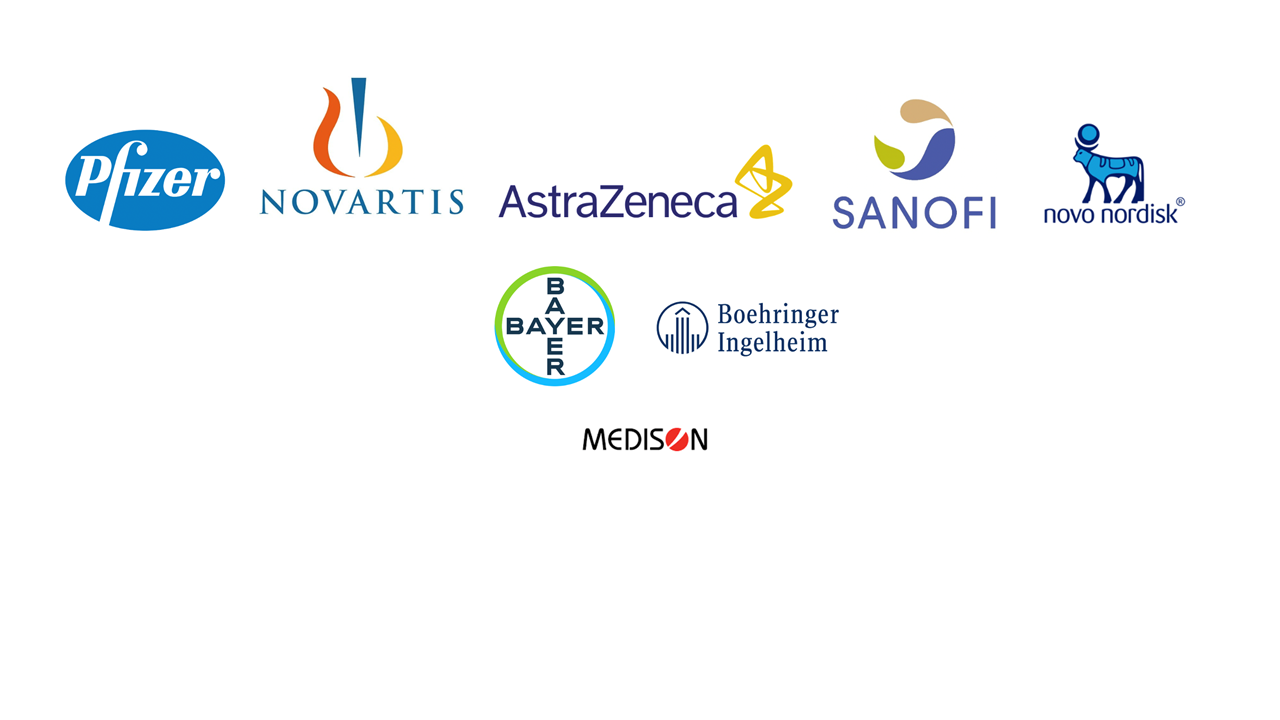
\includegraphics[width=1.2\linewidth]{updated logo page} \end{figure}

\pagebreak

\section{Chapter 1: Acute Coronary Syndrome (ACS) in
Cardiology}\label{chapter-1-acute-coronary-syndrome-acs-in-cardiology}

\subsection{1.1 Distribution of Patients with ACS by Electrocardiogram
(ECG) on
Admission}\label{distribution-of-patients-with-acs-by-electrocardiogram-ecg-on-admission}

~

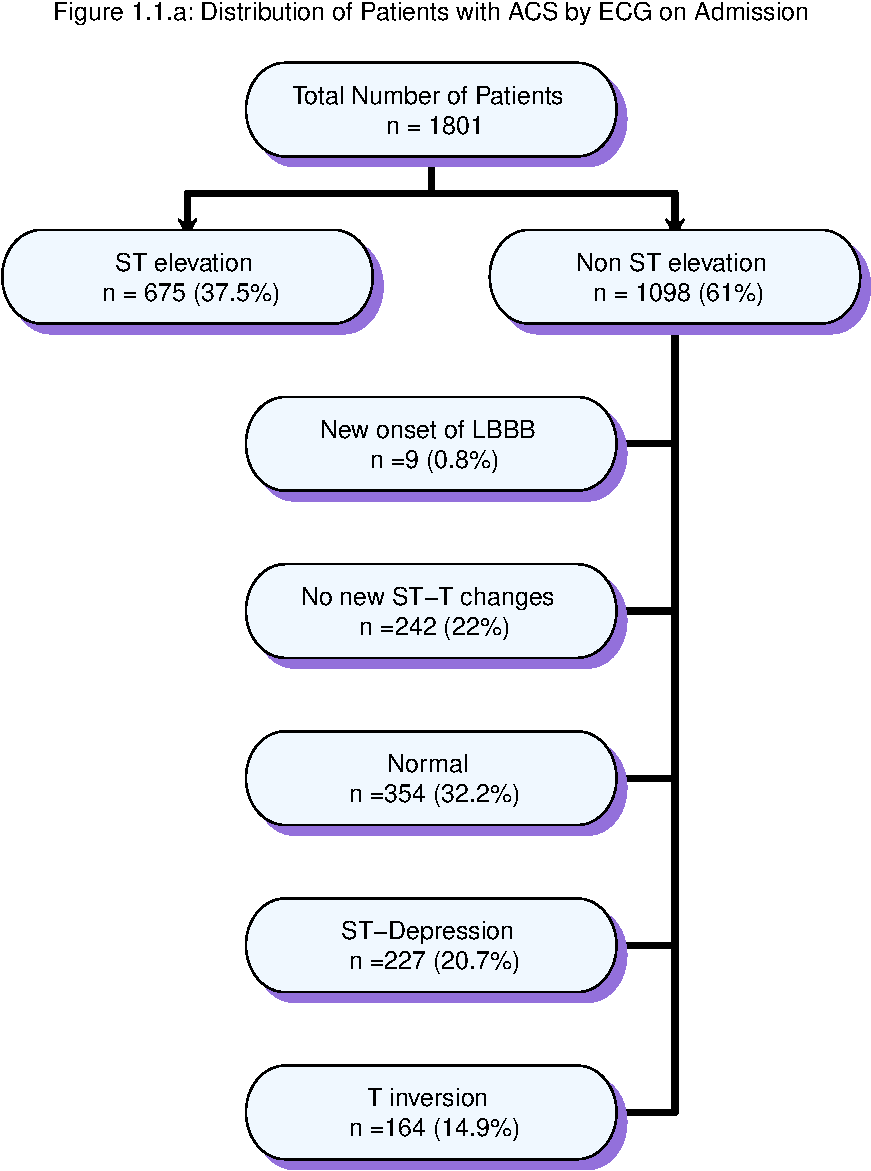
\includegraphics{ACSIS_2024_v1_pdf_files/figure-latex/unnamed-chunk-5-1.pdf}

\pagebreak

~

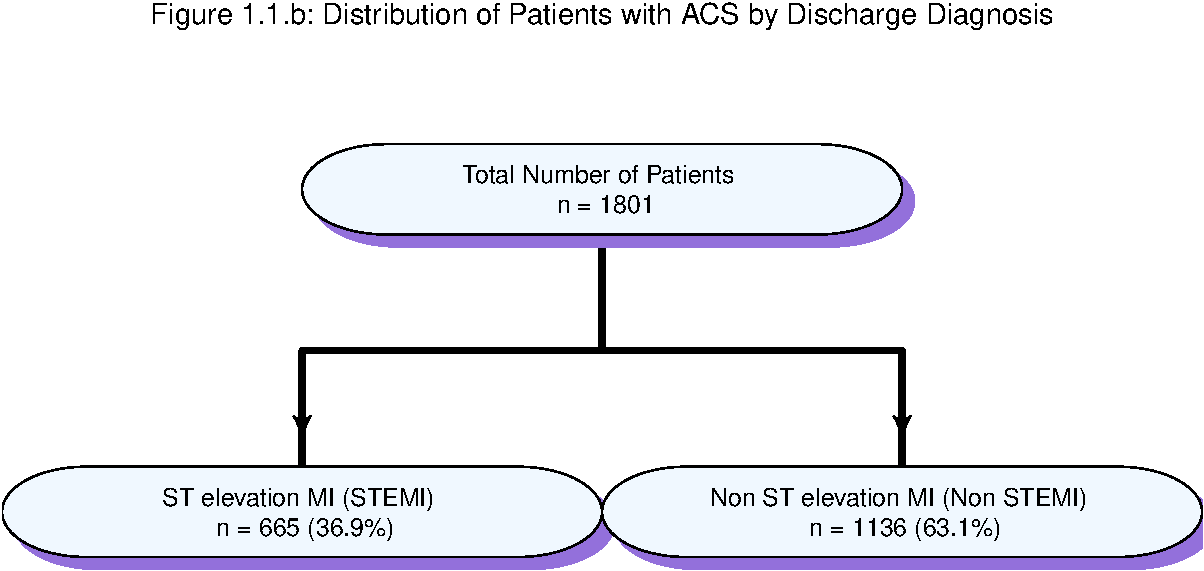
\includegraphics{ACSIS_2024_v1_pdf_files/figure-latex/unnamed-chunk-6-1.pdf}

\pagebreak

~

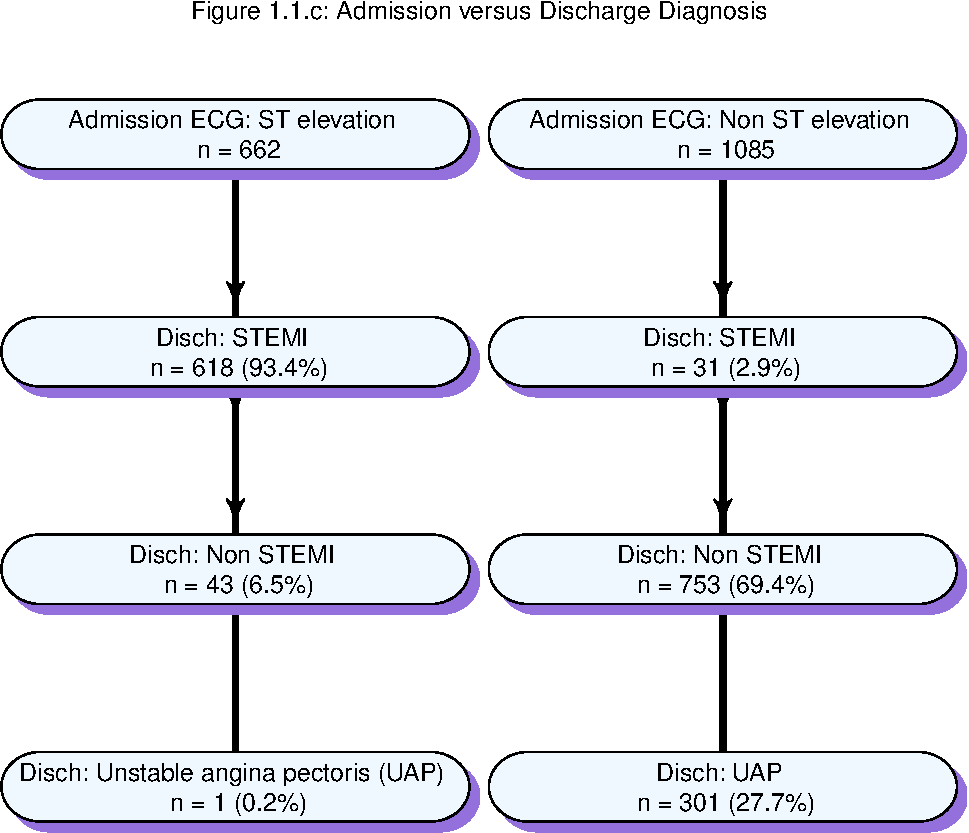
\includegraphics{ACSIS_2024_v1_pdf_files/figure-latex/unnamed-chunk-7-1.pdf}

\pagebreak

\subsection{1.2 Demographic
Characteristics}\label{demographic-characteristics}

\subsubsection{1.2.1 Age Distribution by ECG on
Admission}\label{age-distribution-by-ecg-on-admission}

~

Patients with ST elevation were younger (mean age: 62.7 \(\pm\) 12.1)
than those with non ST elevation (mean age: 66.1 \(\pm\) 11.9), and the
age distribution of patients with ST elevation indicated a greater
proportion of younger patients (55\% were aged \textless{} 65 years)
than that of patients with non ST elevation (44.4\% aged \textless{} 65
years).

~

\begin{table}[H]
\centering
\caption{\label{tab:unnamed-chunk-9}Table 1.1: Age Distribution by ECG on Admission}
\centering
\begin{tabular}[t]{>{\raggedright\arraybackslash}p{3cm}>{\centering\arraybackslash}p{3cm}>{\centering\arraybackslash}p{3cm}>{\centering\arraybackslash}p{3cm}>{\centering\arraybackslash}p{2.5cm}}
\toprule
  & Total & Non ST elevation & ST elevation & p-value\\
\midrule
\cellcolor{gray!10}{n} & \cellcolor{gray!10}{1801} & \cellcolor{gray!10}{1085} & \cellcolor{gray!10}{662} & \cellcolor{gray!10}{}\\
Age groups ($\%$) &  &  &  & <0.001\\
\hspace{1em}\cellcolor{gray!10}{< 50} & \cellcolor{gray!10}{206 (11.4)} & \cellcolor{gray!10}{94 ( 8.7)} & \cellcolor{gray!10}{101 (15.3)} & \cellcolor{gray!10}{}\\
\hspace{1em}50-64 & 669 (37.1) & 388 (35.8) & 263 (39.7) & \\
\hspace{1em}\cellcolor{gray!10}{65-79} & \cellcolor{gray!10}{723 (40.1)} & \cellcolor{gray!10}{457 (42.1)} & \cellcolor{gray!10}{249 (37.6)} & \cellcolor{gray!10}{}\\
\hspace{1em}$\geq$ 80 & 203 (11.3) & 146 (13.5) & 49 ( 7.4) & \\
\cellcolor{gray!10}{Age (mean(sd))} & \cellcolor{gray!10}{64.75 (12.11)} & \cellcolor{gray!10}{66.10 (11.86)} & \cellcolor{gray!10}{62.73 (12.10)} & \cellcolor{gray!10}{<0.001}\\
\bottomrule
\multicolumn{5}{l}{\rule{0pt}{1em}Percentages are calculated out of available data}\\
\end{tabular}
\end{table}

~

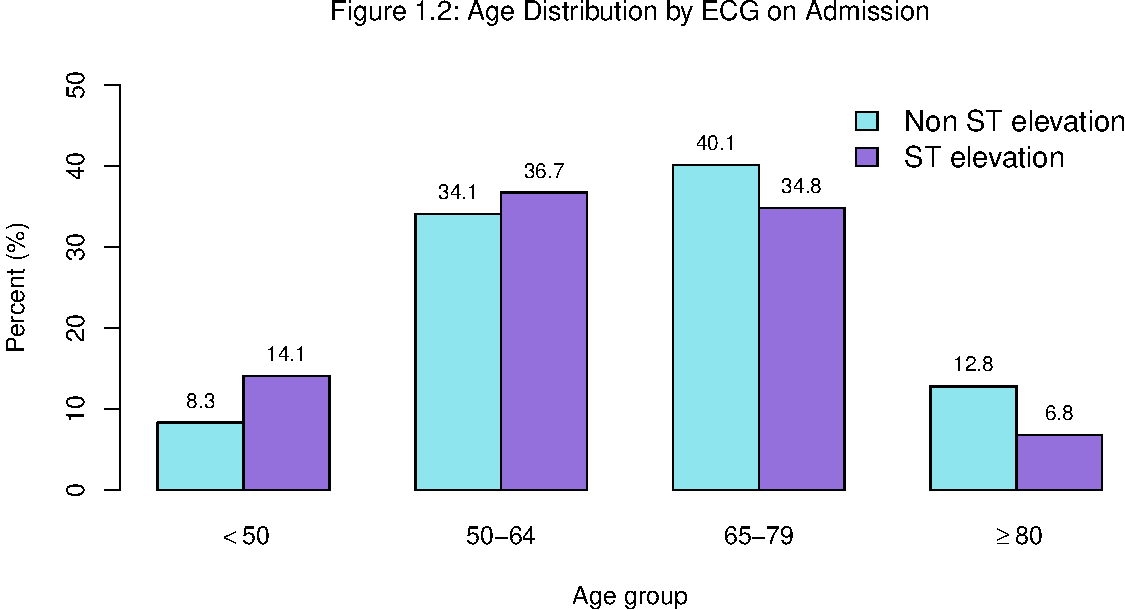
\includegraphics{ACSIS_2024_v1_pdf_files/figure-latex/unnamed-chunk-10-1.pdf}

\pagebreak

\subsubsection{1.2.2 Age Distribution by
Gender}\label{age-distribution-by-gender}

~

The age distribution of male patients was significantly different from
that of female patients. The majority of men (52.6\%) were in the
younger age groups (\textless{} 65) and only 9.2\% were aged 80 or
above. 12.8\% of men were less than 50 years old. By contrast, the
majority of the female patients were in the older age groups \(\geq 65\)
(68.7\%). The number of women under the age of 50 was significantly
lower than of their male counterparts (5.6\%), and 20.4\% were aged 80
or above.

~

\begin{table}[H]
\centering
\caption{\label{tab:unnamed-chunk-12}Table 1.2: Age Distribution by Gender}
\centering
\begin{tabular}[t]{>{\raggedright\arraybackslash}p{3cm}>{\centering\arraybackslash}p{3cm}>{\centering\arraybackslash}p{3cm}>{\centering\arraybackslash}p{3cm}>{\centering\arraybackslash}p{2.5cm}}
\toprule
  & Total & Women & Men & p-value\\
\midrule
\cellcolor{gray!10}{n} & \cellcolor{gray!10}{1801} & \cellcolor{gray!10}{339} & \cellcolor{gray!10}{1461} & \cellcolor{gray!10}{}\\
Age groups ($\%$) &  &  &  & <0.001\\
\hspace{1em}\cellcolor{gray!10}{< 50} & \cellcolor{gray!10}{206 (11.4)} & \cellcolor{gray!10}{19 ( 5.6)} & \cellcolor{gray!10}{187 (12.8)} & \cellcolor{gray!10}{}\\
\hspace{1em}50-64 & 669 (37.1) & 87 (25.7) & 581 (39.8) & \\
\hspace{1em}\cellcolor{gray!10}{65-79} & \cellcolor{gray!10}{723 (40.1)} & \cellcolor{gray!10}{164 (48.4)} & \cellcolor{gray!10}{559 (38.3)} & \cellcolor{gray!10}{}\\
\hspace{1em}$\geq$ 80 & 203 (11.3) & 69 (20.4) & 134 ( 9.2) & \\
\cellcolor{gray!10}{Age (mean(sd))} & \cellcolor{gray!10}{64.75 (12.11)} & \cellcolor{gray!10}{69.87 (11.63)} & \cellcolor{gray!10}{63.57 (11.91)} & \cellcolor{gray!10}{<0.001}\\
\bottomrule
\multicolumn{5}{l}{\rule{0pt}{1em}Percentages are calculated out of available data}\\
\end{tabular}
\end{table}

~

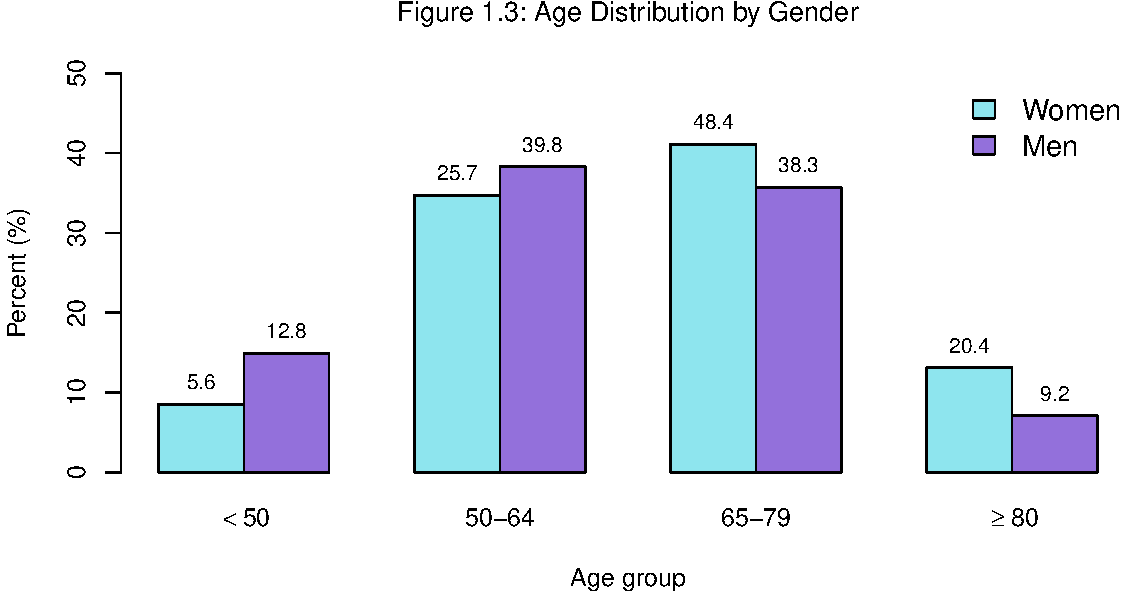
\includegraphics{ACSIS_2024_v1_pdf_files/figure-latex/unnamed-chunk-13-1.pdf}

\pagebreak

\subsubsection{1.2.3 Gender Distribution}\label{gender-distribution}

~

For both STEMI and Non STEMI patients we observed a clear male
predominance.

~

\begin{table}[H]
\centering
\caption{\label{tab:unnamed-chunk-15}Table 1.3: Gender Distribution}
\centering
\begin{tabular}[t]{>{\raggedright\arraybackslash}p{3cm}>{\centering\arraybackslash}p{3cm}>{\centering\arraybackslash}p{3cm}>{\centering\arraybackslash}p{3cm}>{\centering\arraybackslash}p{2.5cm}}
\toprule
  & Total & Non STEMI & STEMI & p-value\\
\midrule
\cellcolor{gray!10}{n} & \cellcolor{gray!10}{1801} & \cellcolor{gray!10}{1151} & \cellcolor{gray!10}{650} & \cellcolor{gray!10}{}\\
Women (\%) & 339 (18.8) & 222 (19.3) & 117 (18.0) & 0.537\\
\cellcolor{gray!10}{Men (\%)} & \cellcolor{gray!10}{1461 (81.2)} & \cellcolor{gray!10}{928 (80.7)} & \cellcolor{gray!10}{533 (82.0)} & \cellcolor{gray!10}{}\\
\bottomrule
\multicolumn{5}{l}{\rule{0pt}{1em}Percentages are calculated out of available data}\\
\end{tabular}
\end{table}

~

~

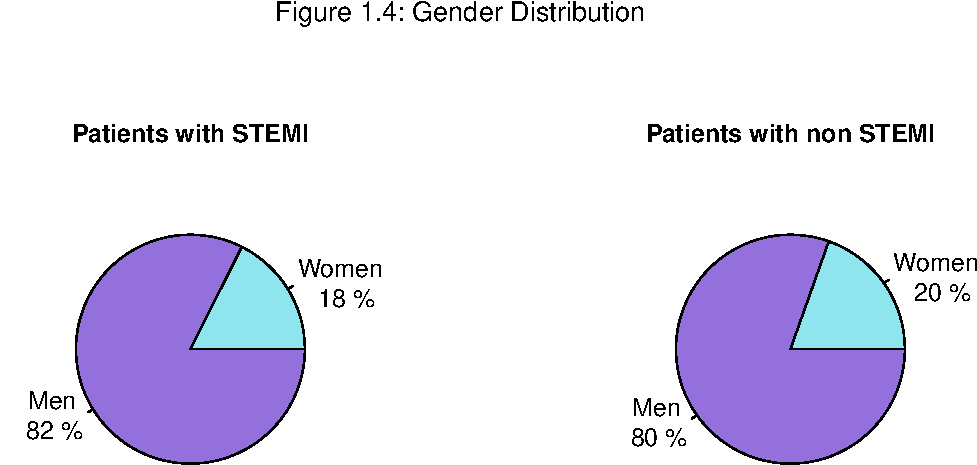
\includegraphics{ACSIS_2024_v1_pdf_files/figure-latex/unnamed-chunk-16-1.pdf}

\pagebreak

\subsection{1.3 Cardiovascular History}\label{cardiovascular-history}

\subsubsection{1.3.1 Cardiovascular
History}\label{cardiovascular-history-1}

A history of ACS, cardiomyopathy, congestive heart failure (CHF),
chronic renal failure, peripheral artery disease (PAD) and atrial
fibrillation was significantly more frequent among patients with non
STEMI. Similarly, more patients with non STEMI had undergone
percutaneous coronary intervention (PCI) or coronary artery bypass
grafting (CABG) prior to hospitalization.

~

\begin{table}[H]
\centering
\caption{\label{tab:unnamed-chunk-18}Table 1.4: Prior Cardiovascular History}
\centering
\begin{tabular}[t]{>{\raggedright\arraybackslash}p{7cm}>{\centering\arraybackslash}p{2cm}>{\centering\arraybackslash}p{2cm}>{\centering\arraybackslash}p{2cm}>{\centering\arraybackslash}p{2cm}}
\toprule
  & Total & Non STEMI & STEMI & p-value\\
\midrule
\cellcolor{gray!10}{n} & \cellcolor{gray!10}{1801} & \cellcolor{gray!10}{1151} & \cellcolor{gray!10}{650} & \cellcolor{gray!10}{}\\
ACS ($\%$) & 655 (37.5) & 486 (44.3) & 169 (26.1) & <0.001\\
\cellcolor{gray!10}{CABG ($\%$)} & \cellcolor{gray!10}{100 ( 5.7)} & \cellcolor{gray!10}{86 ( 7.8)} & \cellcolor{gray!10}{14 ( 2.2)} & \cellcolor{gray!10}{<0.001}\\
PCI ($\%$) & 636 (36.3) & 476 (43.2) & 160 (24.7) & <0.001\\
\cellcolor{gray!10}{Cardiomyopathy ($\%$)} & \cellcolor{gray!10}{97 ( 5.6)} & \cellcolor{gray!10}{78 ( 7.1)} & \cellcolor{gray!10}{19 ( 2.9)} & \cellcolor{gray!10}{<0.001}\\
CHF ($\%$) & 154 ( 8.8) & 125 (11.4) & 29 ( 4.5) & <0.001\\
\cellcolor{gray!10}{Chronic Kidney Disease (CKD) ($\%$)} & \cellcolor{gray!10}{182 (10.4)} & \cellcolor{gray!10}{139 (12.7)} & \cellcolor{gray!10}{43 ( 6.6)} & \cellcolor{gray!10}{<0.001}\\
PAD ($\%$) & 100 ( 5.8) & 76 ( 6.9) & 24 ( 3.7) & 0.008\\
\cellcolor{gray!10}{Stroke/Transient ischemic attack (TIA) ($\%$)} & \cellcolor{gray!10}{157 ( 9.0)} & \cellcolor{gray!10}{104 ( 9.5)} & \cellcolor{gray!10}{53 ( 8.2)} & \cellcolor{gray!10}{0.401}\\
Chronic Obstructive Pulmonary Disease (COPD) ($\%$) & 113 ( 6.5) & 81 ( 7.4) & 32 ( 4.9) & 0.055\\
\cellcolor{gray!10}{Atrial fibrillation/Flutter ($\%$)} & \cellcolor{gray!10}{104 ( 5.9)} & \cellcolor{gray!10}{85 ( 7.7)} & \cellcolor{gray!10}{19 ( 2.9)} & \cellcolor{gray!10}{<0.001}\\
Implantable cardioverter-defibrillators (ICD)/Cardiac resynchronization therapy (CRT) implant ($\%$) & 34 ( 2.1) & 28 ( 2.8) & 6 ( 1.0) & 0.023\\
\cellcolor{gray!10}{Any malignancy ($\%$)} & \cellcolor{gray!10}{107 ( 6.6)} & \cellcolor{gray!10}{75 ( 7.4)} & \cellcolor{gray!10}{32 ( 5.1)} & \cellcolor{gray!10}{0.087}\\
Thyroid disease ($\%$) & 72 ( 4.4) & 52 ( 5.2) & 20 ( 3.2) & 0.089\\
\bottomrule
\multicolumn{5}{l}{\rule{0pt}{1em}Percentages are calculated out of available data}\\
\end{tabular}
\end{table}

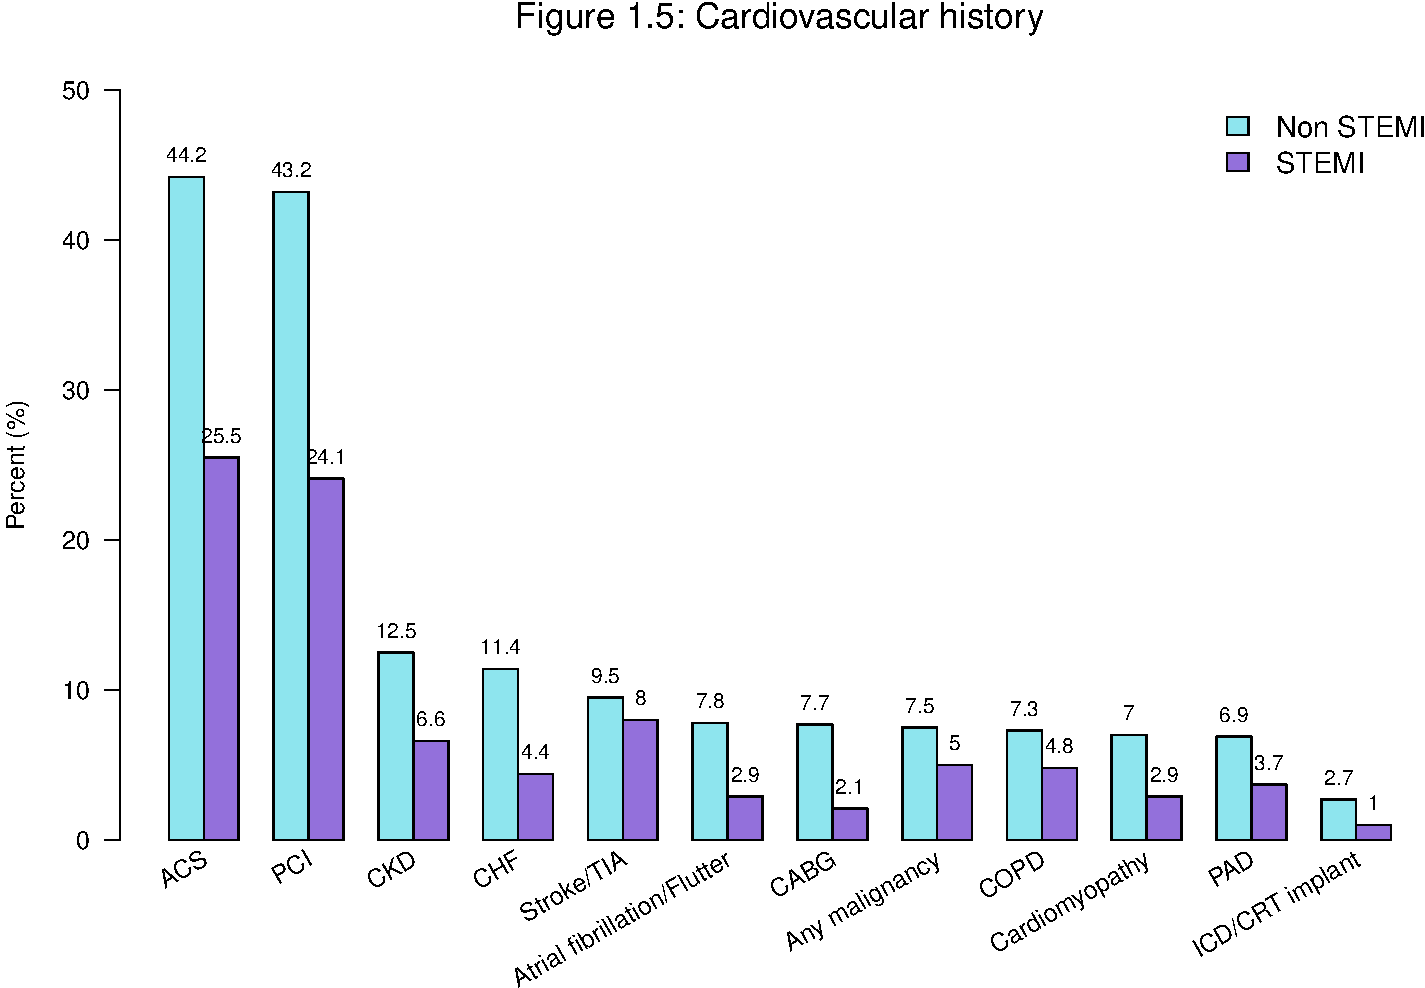
\includegraphics{ACSIS_2024_v1_pdf_files/figure-latex/unnamed-chunk-19-1.pdf}

\pagebreak

\subsubsection{1.3.2 Risk Factors}\label{risk-factors}

Current smoking was more prevalent among patients presenting with STEMI,
while other risk factors were generally more prevalent among patients
presenting with non STEMI. The rates of newly diagnosed diabetes were
higher among those with STEMI. No difference was found in the prevalence
of family history of coronary artery disease (CAD).

~

\begin{table}[H]
\centering
\caption{\label{tab:unnamed-chunk-21}Table 1.5: Risk Factors}
\centering
\begin{tabular}[t]{>{\raggedright\arraybackslash}p{5cm}>{\centering\arraybackslash}p{2.5cm}>{\centering\arraybackslash}p{2.5cm}>{\centering\arraybackslash}p{2.5cm}>{\centering\arraybackslash}p{2cm}}
\toprule
  & Total & Non STEMI & STEMI & p-value\\
\midrule
\cellcolor{gray!10}{n} & \cellcolor{gray!10}{1801} & \cellcolor{gray!10}{1151} & \cellcolor{gray!10}{650} & \cellcolor{gray!10}{}\\
Hypertension (\%) & 1144 (65.6) & 802 (73.1) & 342 (52.8) & <0.001\\
\cellcolor{gray!10}{Diabetes (\%)} & \cellcolor{gray!10}{754 (43.0)} & \cellcolor{gray!10}{527 (47.8)} & \cellcolor{gray!10}{227 (34.9)} & \cellcolor{gray!10}{<0.001}\\
\hspace{1em}* Newly diagnosed (\%) & 31 ( 4.1) & 18 ( 3.4) & 13 ( 5.7) & 0.205\\
\cellcolor{gray!10}{Dyslipidemia (\%)} & \cellcolor{gray!10}{1326 (76.0)} & \cellcolor{gray!10}{870 (79.3)} & \cellcolor{gray!10}{456 (70.5)} & \cellcolor{gray!10}{<0.001}\\
Current smoker (\%) & 686 (38.1) & 378 (32.8) & 308 (47.4) & <0.001\\
\cellcolor{gray!10}{Past smoker (\%)} & \cellcolor{gray!10}{314 (17.4)} & \cellcolor{gray!10}{220 (19.1)} & \cellcolor{gray!10}{94 (14.5)} & \cellcolor{gray!10}{0.015}\\
Family history of CAD (\%) & 445 (30.5) & 271 (29.7) & 174 (31.9) & 0.400\\
\bottomrule
\multicolumn{5}{l}{\rule{0pt}{1em}Percentages are calculated out of available data}\\
\multicolumn{5}{l}{\rule{0pt}{1em}Newly diagnosed expressed as percentage of total patients with specific risk factor}\\
\end{tabular}
\end{table}

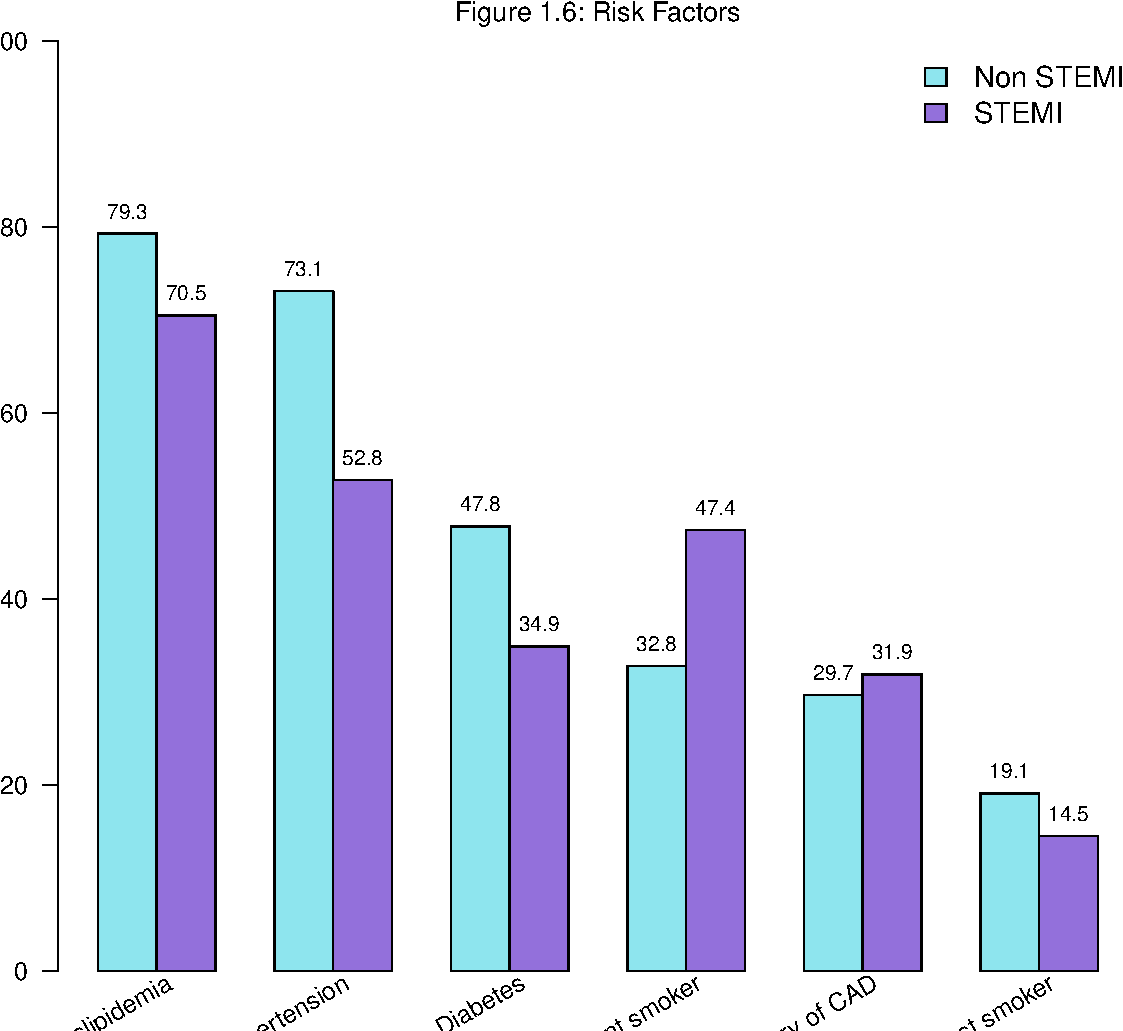
\includegraphics{ACSIS_2024_v1_pdf_files/figure-latex/unnamed-chunk-22-1.pdf}

\pagebreak

\subsection{1.4 Prior Chronic Treatment}\label{prior-chronic-treatment}

Prior to the index hospitalization, a higher proportion of patients with
non STEMI (40.6\%) were being treated with aspirin compared to those
with STEMI (27.2\%). Other drugs in common use were
Angiotensin-Converting-Enzyme (ACE) Inhibitors and Angiotensin Receptor
Blockers (ARB), Beta Blockers, lipid-lowering drugs (primarily statins)
and diuretics all of which were in use more frequently among patients
presenting with non STEMI. 7.6\% of patients with non STEMI and 2.5\% of
those with STEMI were being treated with clopidogrel.

~

\begin{ThreePartTable}
\begin{TableNotes}
\item[1] Oral anticoagulants include: Warfarin, Dabigatran, Rivaroxaban, Apixaban
\item[2] Direct Oral anticoagulants include: Dabigatran, Rivaroxaban, Apixaban
\item[3] Antihyperglycemic drugs include: Glibenclamide, Glipizide, Glimepiride, Metformin, Sitagliptine, Saxagliptine, Vidagliptine, Linagliptine, Exenatide, Liraglutide, Dapagliflozin, Acarbose, Meglinitides, TZDs, Rosiglitazone
\item[4] Statins include: Simvastatin, Pravastatin, Atorvastatin, Rosuvastatin
\item[*] Percentages are calculated out of available data
\end{TableNotes}
\begin{longtable}[t]{>{\raggedright\arraybackslash}p{5cm}>{\centering\arraybackslash}p{2.5cm}>{\centering\arraybackslash}p{2.5cm}>{\centering\arraybackslash}p{2.5cm}>{\centering\arraybackslash}p{2cm}}
\caption{\label{tab:unnamed-chunk-24}Table 1.6: Prior Chronic Treatment}\\
\toprule
  & Total & Non STEMI & STEMI & p-value\\
\midrule
\cellcolor{gray!10}{n} & \cellcolor{gray!10}{1801} & \cellcolor{gray!10}{1151} & \cellcolor{gray!10}{650} & \cellcolor{gray!10}{}\\
\addlinespace[0.3em]
\multicolumn{5}{l}{\textbf{Anti-platelets}}\\
\hspace{1em}Aspirin ($\%$) & 644 (35.8) & 467 (40.6) & 177 (27.2) & <0.001\\
\hspace{1em}\cellcolor{gray!10}{P2Y12 ($\%$)} & \cellcolor{gray!10}{163 ( 9.1)} & \cellcolor{gray!10}{132 (11.5)} & \cellcolor{gray!10}{31 ( 4.8)} & \cellcolor{gray!10}{<0.001}\\
\hspace{1em}Clopidogrel ($\%$) & 104 ( 5.8) & 88 ( 7.6) & 16 ( 2.5) & <0.001\\
\hspace{1em}\cellcolor{gray!10}{Prasugrel ($\%$)} & \cellcolor{gray!10}{27 ( 1.5)} & \cellcolor{gray!10}{19 ( 1.7)} & \cellcolor{gray!10}{8 ( 1.2)} & \cellcolor{gray!10}{0.615}\\
\hspace{1em}Ticagrelor ($\%$) & 32 ( 1.8) & 25 ( 2.2) & 7 ( 1.1) & 0.133\\
\addlinespace[0.3em]
\multicolumn{5}{l}{\textbf{Anticoagulants}}\\
\hspace{1em}\cellcolor{gray!10}{Oral anticoagulants\textsuperscript{1}($\%$)} & \cellcolor{gray!10}{88 ( 4.9)} & \cellcolor{gray!10}{71 ( 6.2)} & \cellcolor{gray!10}{17 ( 2.6)} & \cellcolor{gray!10}{0.001}\\
\hspace{1em}Direct oral anticoagulation (DOAC)\textsuperscript{2}($\%$) & 80 ( 4.4) & 64 ( 5.6) & 16 ( 2.5) & 0.003\\
\hspace{1em}\cellcolor{gray!10}{Warfarin ($\%$)} & \cellcolor{gray!10}{9 ( 0.5)} & \cellcolor{gray!10}{8 ( 0.7)} & \cellcolor{gray!10}{1 ( 0.2)} & \cellcolor{gray!10}{0.224}\\
\hspace{1em}Dabigatran ($\%$) & 4 ( 0.2) & 2 ( 0.2) & 2 ( 0.3) & 0.953\\
\hspace{1em}\cellcolor{gray!10}{Rivaroxaban ($\%$)} & \cellcolor{gray!10}{14 ( 0.8)} & \cellcolor{gray!10}{9 ( 0.8)} & \cellcolor{gray!10}{5 ( 0.8)} & \cellcolor{gray!10}{1.000}\\
\hspace{1em}Apixaban ($\%$) & 62 ( 3.4) & 53 ( 4.6) & 9 ( 1.4) & 0.001\\
\addlinespace[0.3em]
\multicolumn{5}{l}{\textbf{Other}}\\
\hspace{1em}\cellcolor{gray!10}{ACE-I ($\%$)} & \cellcolor{gray!10}{331 (18.4)} & \cellcolor{gray!10}{245 (21.3)} & \cellcolor{gray!10}{86 (13.2)} & \cellcolor{gray!10}{<0.001}\\
\hspace{1em}ARB ($\%$) & 244 (13.5) & 172 (14.9) & 72 (11.1) & 0.026\\
\hspace{1em}\cellcolor{gray!10}{Beta Blockers ($\%$)} & \cellcolor{gray!10}{445 (24.7)} & \cellcolor{gray!10}{333 (28.9)} & \cellcolor{gray!10}{112 (17.2)} & \cellcolor{gray!10}{<0.001}\\
\hspace{1em}Calcium channel blockers (CCB) ($\%$) & 219 (12.2) & 168 (14.6) & 51 ( 7.8) & <0.001\\
\hspace{1em}\cellcolor{gray!10}{Nitrates ($\%$)} & \cellcolor{gray!10}{21 ( 1.2)} & \cellcolor{gray!10}{20 ( 1.7)} & \cellcolor{gray!10}{1 ( 0.2)} & \cellcolor{gray!10}{0.005}\\
\hspace{1em}Diuretics ($\%$) & 115 ( 6.4) & 97 ( 8.4) & 18 ( 2.8) & <0.001\\
\hspace{1em}\cellcolor{gray!10}{Antihyperglycemic drugs\textsuperscript{3} ($\%$)} & \cellcolor{gray!10}{270 (15.0)} & \cellcolor{gray!10}{194 (16.9)} & \cellcolor{gray!10}{76 (11.7)} & \cellcolor{gray!10}{0.004}\\
\hspace{1em}Statins\textsuperscript{4} ($\%$) & 665 (36.9) & 476 (41.4) & 189 (29.1) & <0.001\\
\hspace{1em}\cellcolor{gray!10}{Ezetimibe ($\%$)} & \cellcolor{gray!10}{165 ( 9.2)} & \cellcolor{gray!10}{129 (11.2)} & \cellcolor{gray!10}{36 ( 5.5)} & \cellcolor{gray!10}{<0.001}\\
\bottomrule
\insertTableNotes
\end{longtable}
\end{ThreePartTable}

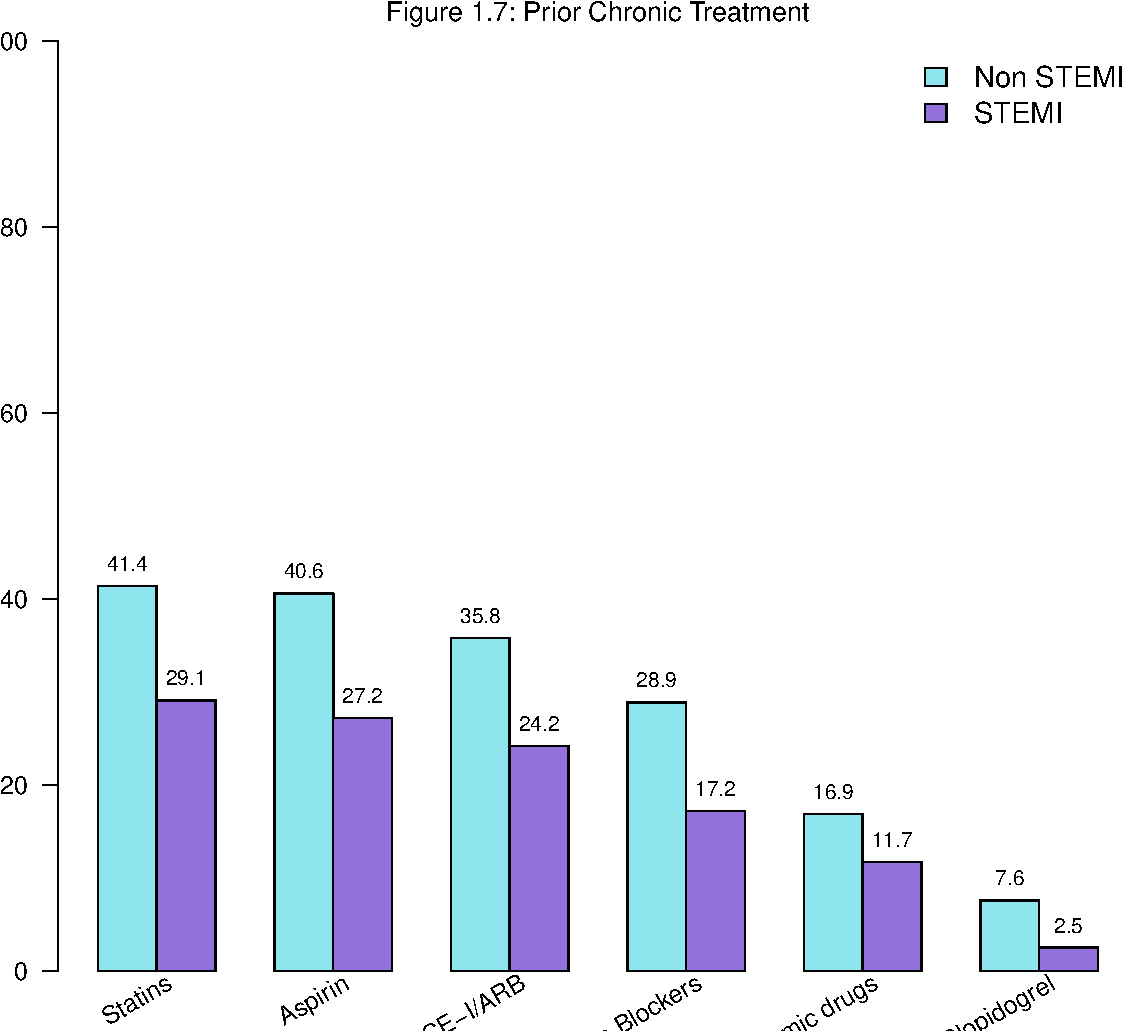
\includegraphics{ACSIS_2024_v1_pdf_files/figure-latex/unnamed-chunk-25-1.pdf}

\pagebreak

\subsection{1.5 Transportation, Pre-Admission and Admission
Information}\label{transportation-pre-admission-and-admission-information}

\subsubsection{1.5.1 Mode of Transportation by ECG on
Admission}\label{mode-of-transportation-by-ecg-on-admission}

41.4\% of all patients arrived at the hospital by means of private
transportation. Patients with ST elevation were more frequently
transported to hospital with mobile intensive care unit (MICU), and
patients with non ST elevation arrived more frequently by means of
private transportation.

~

\begin{table}[H]
\centering
\caption{\label{tab:unnamed-chunk-27}Table 1.7: Mode of Transportation by ECG on Admission}
\centering
\begin{tabular}[t]{>{\raggedright\arraybackslash}p{4.9cm}>{\centering\arraybackslash}p{3.2cm}>{\centering\arraybackslash}p{3.2cm}>{\centering\arraybackslash}p{3.2cm}}
\toprule
  & Total & Non ST elevation & ST elevation\\
\midrule
\cellcolor{gray!10}{n\textsuperscript{1}} & \cellcolor{gray!10}{1450} & \cellcolor{gray!10}{863} & \cellcolor{gray!10}{584}\\
MICU ($\%$) & 622 (42.9) & 244 (28.3) & 378 (64.7)\\
\cellcolor{gray!10}{Private car/ independently ($\%$)} & \cellcolor{gray!10}{601 (41.4)} & \cellcolor{gray!10}{470 (54.5)} & \cellcolor{gray!10}{130 (22.3)}\\
Regular ambulance ($\%$) & 227 (15.7) & 149 (17.3) & 76 (13.0)\\
\bottomrule
\multicolumn{4}{l}{\rule{0pt}{1em}p-value <0.001}\\
\multicolumn{4}{l}{\rule{0pt}{1em}\textsuperscript{1} Excluded in-patients}\\
\end{tabular}
\end{table}

~

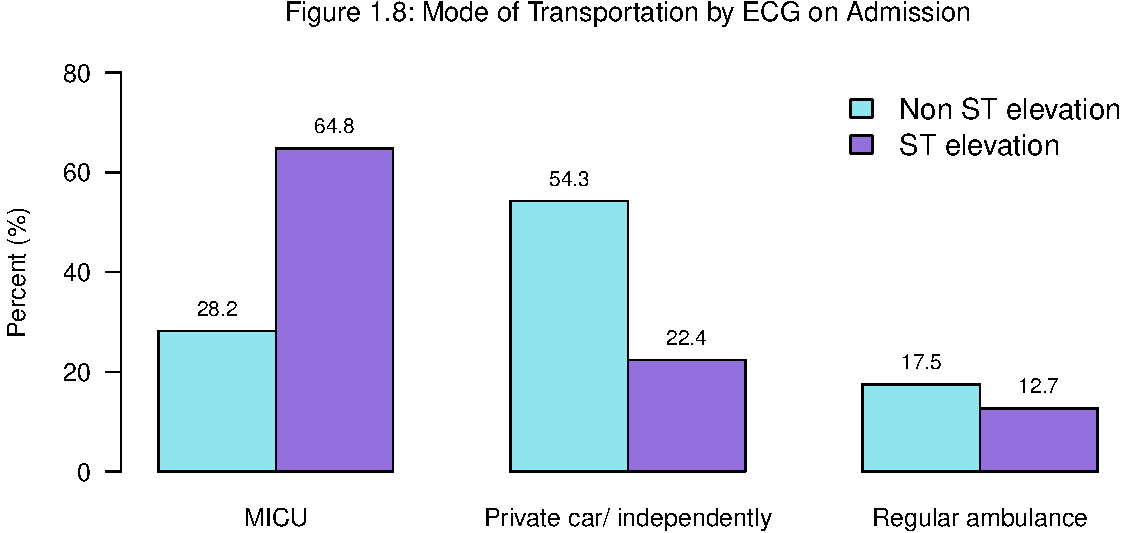
\includegraphics{ACSIS_2024_v1_pdf_files/figure-latex/unnamed-chunk-28-1.pdf}

\pagebreak

\subsubsection{1.5.2 Mode of Transportation by
Gender}\label{mode-of-transportation-by-gender}

NA\% of patients, both men and women, arrived by means of a MICU. Women
were more frequently transported to hospital with regular ambulance and
men arrived more frequently by means of private transportation.

~

\begin{table}[H]
\centering
\caption{\label{tab:unnamed-chunk-30}Table 1.8: Mode of Transportation by Gender}
\centering
\begin{tabular}[t]{>{\raggedright\arraybackslash}p{4.9cm}>{\centering\arraybackslash}p{3.2cm}>{\centering\arraybackslash}p{3.2cm}>{\centering\arraybackslash}p{3.2cm}}
\toprule
  & Total & Women & Men\\
\midrule
\cellcolor{gray!10}{n\textsuperscript{1}} & \cellcolor{gray!10}{1450} & \cellcolor{gray!10}{268} & \cellcolor{gray!10}{1181}\\
MICU ($\%$) & 622 (42.9) & 122 (45.5) & 499 (42.3)\\
\cellcolor{gray!10}{Private car/ independently ($\%$)} & \cellcolor{gray!10}{601 (41.4)} & \cellcolor{gray!10}{101 (37.7)} & \cellcolor{gray!10}{500 (42.3)}\\
Regular ambulance ($\%$) & 227 (15.7) & 45 (16.8) & 182 (15.4)\\
\bottomrule
\multicolumn{4}{l}{\rule{0pt}{1em}p-value = 0.377}\\
\multicolumn{4}{l}{\rule{0pt}{1em}\textsuperscript{1} Excluded in-patients}\\
\end{tabular}
\end{table}

~

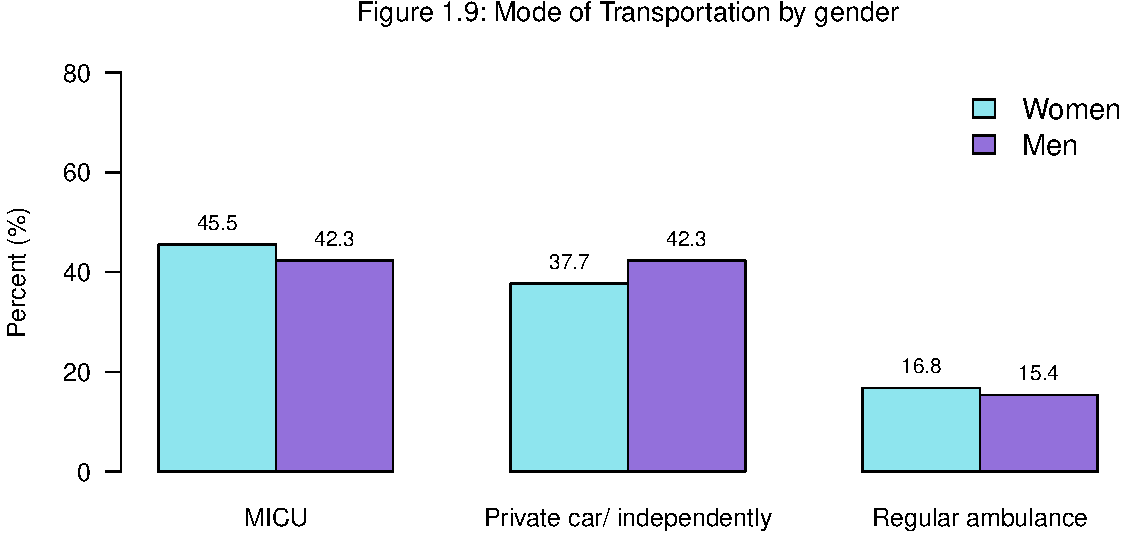
\includegraphics{ACSIS_2024_v1_pdf_files/figure-latex/unnamed-chunk-31-1.pdf}

\pagebreak

\subsubsection{1.5.3 Drugs administered at the Emergency Department
(ED)}\label{drugs-administered-at-the-emergency-department-ed}

~

\begin{table}[H]
\centering
\caption{\label{tab:unnamed-chunk-33}Table 1.9: Drugs administered at the ED}
\centering
\begin{tabular}[t]{>{\raggedright\arraybackslash}p{8cm}>{\centering\arraybackslash}p{2cm}>{\centering\arraybackslash}p{2cm}>{\centering\arraybackslash}p{2cm}>{\centering\arraybackslash}p{2cm}}
\toprule
  & Total & Non ST elevation & ST elevation & p-value\\
\midrule
\cellcolor{gray!10}{n} & \cellcolor{gray!10}{1801} & \cellcolor{gray!10}{1085} & \cellcolor{gray!10}{662} & \cellcolor{gray!10}{}\\
Aspirin (\%) & 645 (49.7) & 458 (45.5) & 187 (64.7) & <0.001\\
\cellcolor{gray!10}{Clopidogrel (\%)} & \cellcolor{gray!10}{69 ( 5.3)} & \cellcolor{gray!10}{51 ( 5.1)} & \cellcolor{gray!10}{18 ( 6.2)} & \cellcolor{gray!10}{0.532}\\
Prasugrel (\%) & 44 ( 3.4) & 15 ( 1.5) & 29 (10.0) & <0.001\\
\cellcolor{gray!10}{Ticagrelor (\%)} & \cellcolor{gray!10}{43 ( 3.3)} & \cellcolor{gray!10}{20 ( 2.0)} & \cellcolor{gray!10}{23 ( 8.0)} & \cellcolor{gray!10}{<0.001}\\
Heparin (\%) & 275 (21.2) & 136 (13.5) & 139 (48.1) & <0.001\\
\cellcolor{gray!10}{Low Molecular Weight Heparin (LMWH) (\%)} & \cellcolor{gray!10}{74 ( 5.7)} & \cellcolor{gray!10}{61 ( 6.1)} & \cellcolor{gray!10}{13 ( 4.5)} & \cellcolor{gray!10}{0.386}\\
\bottomrule
\end{tabular}
\end{table}

~

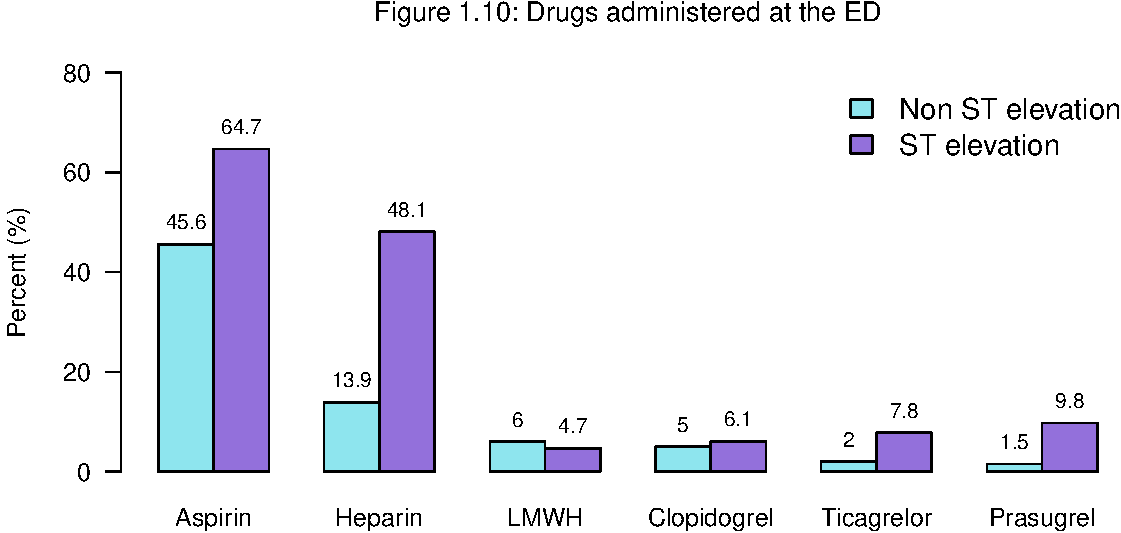
\includegraphics{ACSIS_2024_v1_pdf_files/figure-latex/unnamed-chunk-34-1.pdf}

\pagebreak

\subsubsection{1.5.4 Ward of First Arrival by ECG on
Admission}\label{ward-of-first-arrival-by-ecg-on-admission}

Most patients with ACS present to the ED. However, a higher number of
patients with ST elevation presented directly to the intensive cardiac
care unit (ICCU) and the catheterization laboratory than those with non
ST elevation.

~

\begin{table}[H]
\centering
\caption{\label{tab:unnamed-chunk-36}Table 1.10: Ward of First Arrival by ECG on Admission}
\centering
\begin{tabular}[t]{>{\raggedright\arraybackslash}p{5.5cm}>{\centering\arraybackslash}p{3cm}>{\centering\arraybackslash}p{3cm}>{\centering\arraybackslash}p{3cm}}
\toprule
  & Total & Non ST elevation & ST elevation\\
\midrule
\cellcolor{gray!10}{n} & \cellcolor{gray!10}{1801} & \cellcolor{gray!10}{1085} & \cellcolor{gray!10}{662}\\
Directly to cardiology ward (\%) & 20 ( 1.1) & 19 ( 1.8) & 0 ( 0.0)\\
\cellcolor{gray!10}{Directly to cath lab (\%)} & \cellcolor{gray!10}{200 (11.4)} & \cellcolor{gray!10}{16 ( 1.5)} & \cellcolor{gray!10}{183 (27.6)}\\
Directly to ICCU (\%) & 220 (12.6) & 34 ( 3.1) & 186 (28.1)\\
\cellcolor{gray!10}{Directly to internal medicine ward (\%)} & \cellcolor{gray!10}{5 ( 0.3)} & \cellcolor{gray!10}{4 ( 0.4)} & \cellcolor{gray!10}{1 ( 0.2)}\\
\addlinespace[0.3em]
\multicolumn{4}{l}{\textbf{Patients arrived by MICU}}\\
\hspace{1em}ED (\%) & 1297 (74.1) & 1006 (92.7) & 289 (43.7)\\
\hspace{1em}\cellcolor{gray!10}{Other (\%)} & \cellcolor{gray!10}{9 ( 0.5)} & \cellcolor{gray!10}{6 ( 0.6)} & \cellcolor{gray!10}{3 ( 0.5)}\\
\hspace{1em}n & 622 & 244 & 378\\
\hspace{1em}\cellcolor{gray!10}{Directly to cardiology ward (\%)} & \cellcolor{gray!10}{1 ( 0.2)} & \cellcolor{gray!10}{1 ( 0.4)} & \cellcolor{gray!10}{0 ( 0.0)}\\
\hspace{1em}Directly to cath lab (\%) & 146 (23.5) & 3 ( 1.2) & 143 (37.8)\\
\hspace{1em}\cellcolor{gray!10}{Directly to ICCU (\%)} & \cellcolor{gray!10}{160 (25.7)} & \cellcolor{gray!10}{13 ( 5.3)} & \cellcolor{gray!10}{147 (38.9)}\\
\hspace{1em}Directly to internal medicine ward (\%) & 2 ( 0.3) & 1 ( 0.4) & 1 ( 0.3)\\
\hspace{1em}\cellcolor{gray!10}{ED (\%)} & \cellcolor{gray!10}{311 (50.0)} & \cellcolor{gray!10}{226 (92.6)} & \cellcolor{gray!10}{85 (22.5)}\\
\hspace{1em}Other (\%) & 2 ( 0.3) & 0 ( 0.0) & 2 ( 0.5)\\
\bottomrule
\multicolumn{4}{l}{\rule{0pt}{1em}Difference in ward of first arrival, ST elevation vs. non ST elevation, p <0.001}\\
\end{tabular}
\end{table}

\pagebreak

\subsubsection{1.5.5 First Ward of
Admission}\label{first-ward-of-admission}

As expected, the majority of patients presenting with ST elevation were
hospitalized in the ICCU (95.5\%). 46.3\% of the patients who presented
with non ST elevation were admitted to the ICCU and an additional 40\%
to a cardiology department, with the remaining 12.8\% being admitted to
internal medicine departments.

\hfill\break

\begin{table}[H]
\centering
\caption{\label{tab:unnamed-chunk-38}Table 1.11: First Ward of Hospitalization}
\centering
\begin{tabular}[t]{>{\raggedright\arraybackslash}p{4.9cm}>{\centering\arraybackslash}p{3.2cm}>{\centering\arraybackslash}p{3.2cm}>{\centering\arraybackslash}p{3.2cm}}
\toprule
  & Total & Non ST elevation & ST elevation\\
\midrule
\cellcolor{gray!10}{n} & \cellcolor{gray!10}{1801} & \cellcolor{gray!10}{1085} & \cellcolor{gray!10}{662}\\
ICCU (\%) & 1136 (64.9) & 502 (46.3) & 632 (95.5)\\
\cellcolor{gray!10}{Cardiology (\%)} & \cellcolor{gray!10}{459 (26.2)} & \cellcolor{gray!10}{434 (40.0)} & \cellcolor{gray!10}{25 ( 3.8)}\\
Internal medicine (\%) & 144 ( 8.2) & 139 (12.8) & 3 ( 0.5)\\
\cellcolor{gray!10}{Chest pain unit (\%)} & \cellcolor{gray!10}{1 ( 0.1)} & \cellcolor{gray!10}{1 ( 0.1)} & \cellcolor{gray!10}{0 ( 0.0)}\\
Other (\%) & 11 ( 0.6) & 9 ( 0.8) & 2 ( 0.3)\\
\bottomrule
\multicolumn{4}{l}{\rule{0pt}{1em}Difference in first ward of hospitalization, ST elevation vs. non ST elevation, p <0.001}\\
\end{tabular}
\end{table}

~

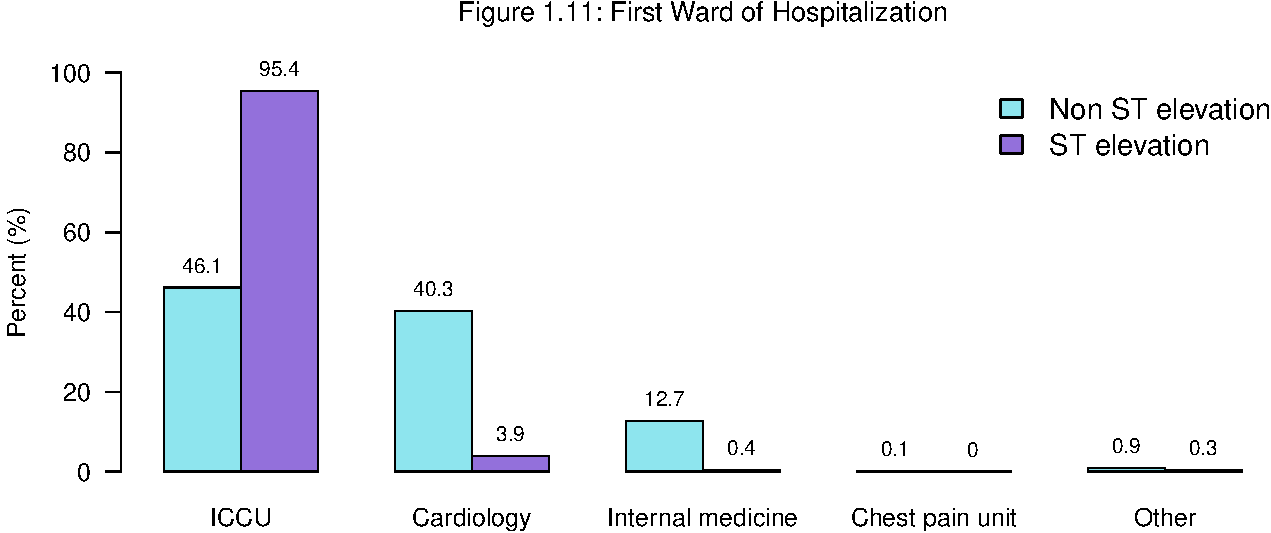
\includegraphics{ACSIS_2024_v1_pdf_files/figure-latex/unnamed-chunk-39-1.pdf}

\pagebreak

\subsubsection{1.5.6 Time from Symptom Onset to Hospital Arrival, by ECG
on
Admission}\label{time-from-symptom-onset-to-hospital-arrival-by-ecg-on-admission}

All time frames were significantly shorter for patients with ST
elevation. Patients with ST elevation sought help earlier when compared
to patients with non ST elevation.

~

\begin{table}[H]
\centering
\caption{\label{tab:unnamed-chunk-41}Table 1.12: Time (minutes) from Symptom Onset to Admission, by ECG on Admission}
\centering
\begin{tabular}[t]{>{\raggedright\arraybackslash}p{3.7cm}>{\centering\arraybackslash}p{3.5cm}>{\centering\arraybackslash}p{3.5cm}>{\centering\arraybackslash}p{3.5cm}>{\centering\arraybackslash}p{1.2cm}}
\toprule
  & Total & Non ST elevation & ST elevation & p-value\\
\midrule
\cellcolor{gray!10}{n\textsuperscript{1}} & \cellcolor{gray!10}{1044} & \cellcolor{gray!10}{499} & \cellcolor{gray!10}{494} & \cellcolor{gray!10}{}\\
Onset to first medical contact, minutes (median [IQR]) & 96.00 [40.00, 290.50] & 120.00 [50.00, 489.75] & 82.00 [30.00, 192.75] & <0.001\\
\cellcolor{gray!10}{First medical contact to arrival, minutes (median [IQR])} & \cellcolor{gray!10}{49.00 [32.00, 75.00]} & \cellcolor{gray!10}{50.00 [34.00, 87.00]} & \cellcolor{gray!10}{47.00 [31.00, 70.00]} & \cellcolor{gray!10}{0.015}\\
Onset to arrival, minutes (median [IQR]) & 153.50 [86.25, 393.75] & 205.00 [97.00, 592.00] & 138.00 [78.00, 257.00] & <0.001\\
\bottomrule
\multicolumn{5}{l}{\rule{0pt}{1em}\textsuperscript{1} Excluded in-patients or patients whose first medical contact was in ED}\\
\end{tabular}
\end{table}

~

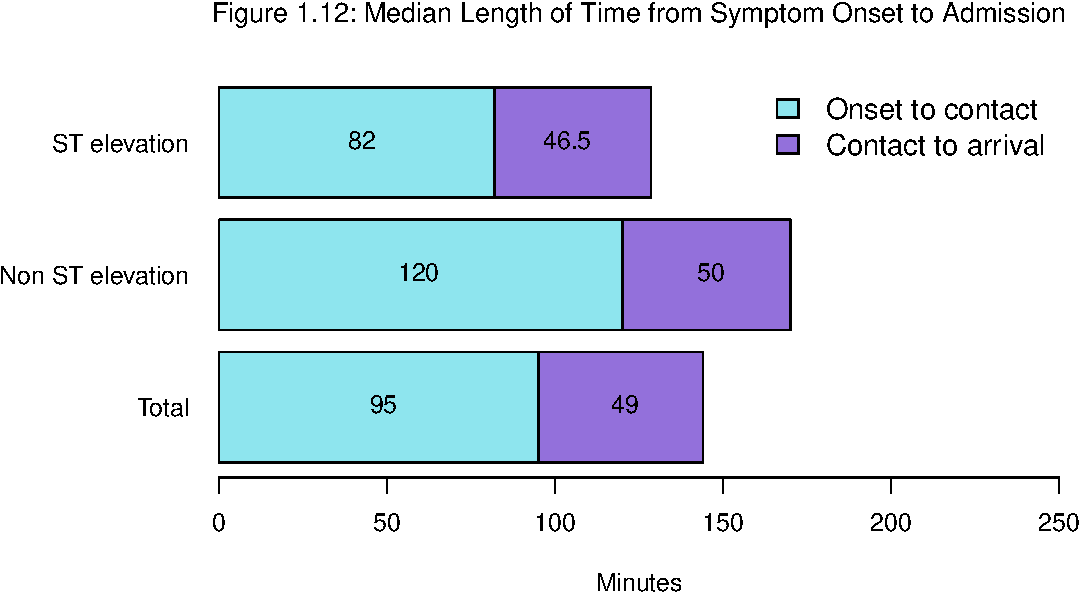
\includegraphics{ACSIS_2024_v1_pdf_files/figure-latex/unnamed-chunk-42-1.pdf}

\pagebreak

\subsubsection{1.5.7 Time from Symptom Onset to Hospital Arrival, by
gender}\label{time-from-symptom-onset-to-hospital-arrival-by-gender}

~

\begin{table}[H]
\centering
\caption{\label{tab:unnamed-chunk-44}Table 1.13: Time (minutes) from Symptom Onset to Admission by gender}
\centering
\begin{tabular}[t]{>{\raggedright\arraybackslash}p{3.7cm}>{\centering\arraybackslash}p{3.3cm}>{\centering\arraybackslash}p{3.3cm}>{\centering\arraybackslash}p{3.3cm}>{\centering\arraybackslash}p{1.5cm}}
\toprule
  & Total & Women & Men & p-value\\
\midrule
\cellcolor{gray!10}{n\textsuperscript{1}} & \cellcolor{gray!10}{1044} & \cellcolor{gray!10}{200} & \cellcolor{gray!10}{843} & \cellcolor{gray!10}{}\\
Onset to first medical contact, minutes (median [IQR]) & 96.00 [40.00, 290.50] & 118.00 [37.00, 390.00] & 90.00 [40.00, 270.00] & 0.508\\
\cellcolor{gray!10}{First medical contact to arrival, minutes (median [IQR])} & \cellcolor{gray!10}{49.00 [32.00, 75.00]} & \cellcolor{gray!10}{52.00 [37.50, 72.50]} & \cellcolor{gray!10}{48.00 [31.00, 76.25]} & \cellcolor{gray!10}{0.256}\\
Onset to arrival, minutes (median [IQR]) & 153.50 [86.25, 393.75] & 174.00 [89.00, 422.50] & 148.00 [86.50, 376.50] & 0.348\\
\bottomrule
\multicolumn{5}{l}{\rule{0pt}{1em}\textsuperscript{1} Excluded in-patients or patients whose first medical contact was in ED}\\
\end{tabular}
\end{table}

~

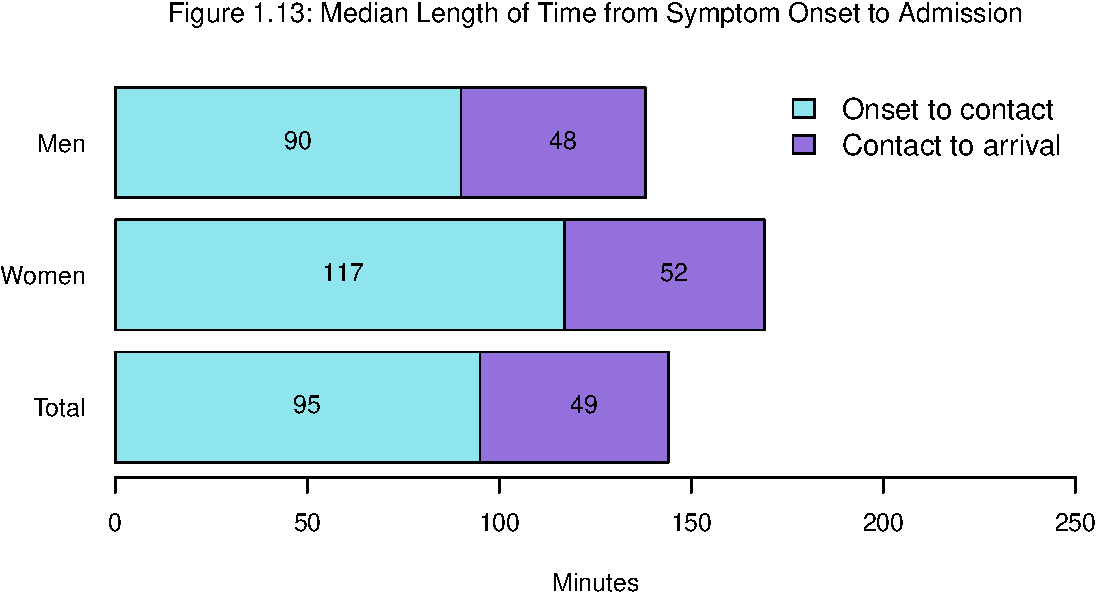
\includegraphics{ACSIS_2024_v1_pdf_files/figure-latex/unnamed-chunk-45-1.pdf}

\pagebreak

\subsubsection{1.5.8 First Medical Contact}\label{first-medical-contact}

41.6\% of patients had the first medical contact at the ED and about
21.5\% at a Health maintenance organization (HMO) primary
clinic/``Moked''. For an additional 22.3\% the primary medical contact
was with MICU. Patients with ST elevation were more likely to have their
first medical contact with a MICU (40\% than those with non ST elevation
(13.2\%).

~

\begin{table}[H]
\centering
\caption{\label{tab:unnamed-chunk-47}Table 1.14: First Medical Contact}
\centering
\begin{tabular}[t]{>{\raggedright\arraybackslash}p{5.5cm}>{\centering\arraybackslash}p{3cm}>{\centering\arraybackslash}p{3cm}>{\centering\arraybackslash}p{3cm}}
\toprule
  & Total & Non ST elevation & ST elevation\\
\midrule
\cellcolor{gray!10}{n} & \cellcolor{gray!10}{1801} & \cellcolor{gray!10}{1085} & \cellcolor{gray!10}{662}\\
ED (\%) & 728 (41.6) & 566 (52.2) & 160 (24.2)\\
\cellcolor{gray!10}{HMO Out Pts. clinic / 'Moked' (\%)} & \cellcolor{gray!10}{377 (21.5)} & \cellcolor{gray!10}{233 (21.5)} & \cellcolor{gray!10}{143 (21.6)}\\
Home visit (\%) & 26 ( 1.5) & 13 ( 1.2) & 13 ( 2.0)\\
\cellcolor{gray!10}{In-patient (\%)} & \cellcolor{gray!10}{29 ( 1.7)} & \cellcolor{gray!10}{20 ( 1.8)} & \cellcolor{gray!10}{8 ( 1.2)}\\
Mobile ICU (\%) & 390 (22.3) & 143 (13.2) & 247 (37.3)\\
\cellcolor{gray!10}{Other hospital (\%)} & \cellcolor{gray!10}{28 ( 1.6)} & \cellcolor{gray!10}{16 ( 1.5)} & \cellcolor{gray!10}{12 ( 1.8)}\\
Regular ambulance (\%) & 173 ( 9.9) & 94 ( 8.7) & 79 (11.9)\\
\bottomrule
\multicolumn{4}{l}{\rule{0pt}{1em}Difference in location of first medical contact, ST elevation vs. non ST elevation, p <0.001}\\
\end{tabular}
\end{table}

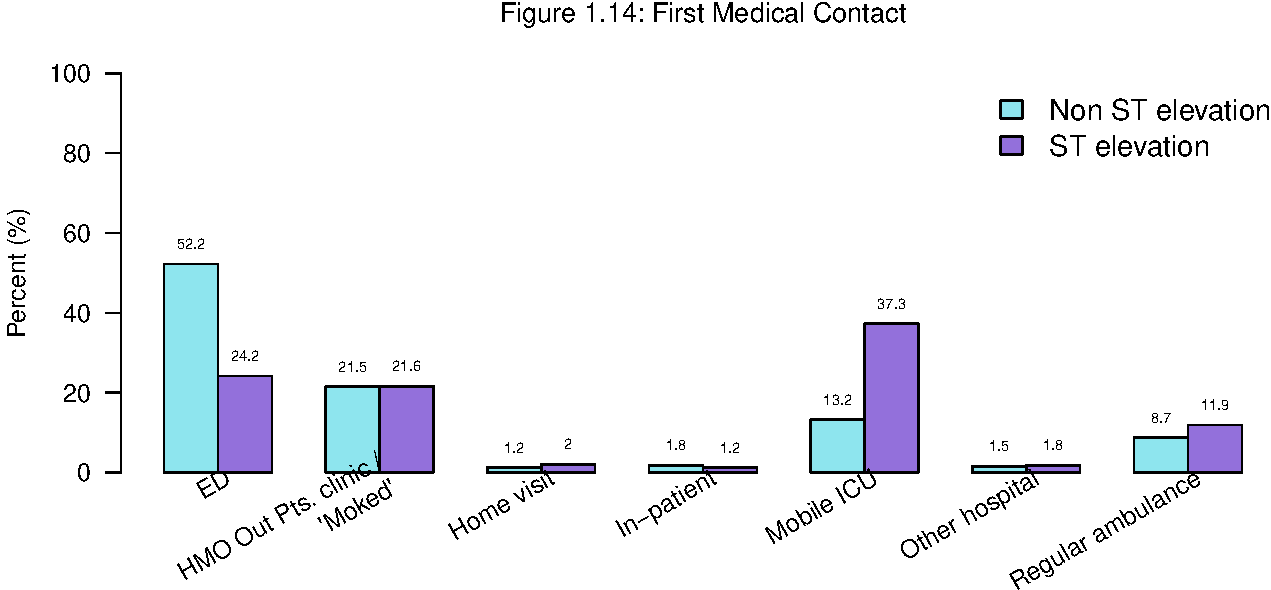
\includegraphics{ACSIS_2024_v1_pdf_files/figure-latex/unnamed-chunk-48-1.pdf}

\pagebreak

\subsubsection{1.5.9 Presenting Symptoms and Killip
Class}\label{presenting-symptoms-and-killip-class}

Typical angina was significantly more frequent in patients presenting
with ST elevation (82\%) than those presenting with non ST elevation
(69\%). However, atypical chest pain was more common in patients
presenting with non ST elevation (11.1\%) than in those with ST
elevation (8\%). Also dyspnea was more common in patients with non ST
elevation (21.8\%) than those with ST elevation (14.7\%).

~

\begin{table}[H]
\centering
\caption{\label{tab:unnamed-chunk-50}Table 1.15: Presenting Symptoms at First Medical Contact}
\centering
\begin{tabular}[t]{>{\raggedright\arraybackslash}p{6cm}>{\centering\arraybackslash}p{3cm}>{\centering\arraybackslash}p{3cm}>{\centering\arraybackslash}p{3cm}>{\centering\arraybackslash}p{1.5cm}}
\toprule
  & Total & Non ST elevation & ST elevation & p-value\\
\midrule
\cellcolor{gray!10}{n} & \cellcolor{gray!10}{1801} & \cellcolor{gray!10}{1085} & \cellcolor{gray!10}{662} & \cellcolor{gray!10}{}\\
Typical angina (\%) & 1296 (72.0) & 749 (69.0) & 543 (82.0) & <0.001\\
\cellcolor{gray!10}{Atypical chest pain (\%)} & \cellcolor{gray!10}{173 ( 9.6)} & \cellcolor{gray!10}{120 (11.1)} & \cellcolor{gray!10}{53 ( 8.0)} & \cellcolor{gray!10}{0.047}\\
Syncope (\%) & 39 ( 2.2) & 22 ( 2.0) & 17 ( 2.6) & 0.566\\
\cellcolor{gray!10}{Aborted Sudden Cardiac Death (SCD) (\%)} & \cellcolor{gray!10}{10 ( 0.6)} & \cellcolor{gray!10}{3 ( 0.3)} & \cellcolor{gray!10}{7 ( 1.1)} & \cellcolor{gray!10}{0.076}\\
Palpitations (\%) & 30 ( 1.7) & 23 ( 2.1) & 6 ( 0.9) & 0.083\\
\cellcolor{gray!10}{Dyspnea (\%)} & \cellcolor{gray!10}{336 (18.7)} & \cellcolor{gray!10}{237 (21.8)} & \cellcolor{gray!10}{97 (14.7)} & \cellcolor{gray!10}{<0.001}\\
Abdominal pain (\%) & 84 ( 4.7) & 46 ( 4.2) & 38 ( 5.7) & 0.191\\
\bottomrule
\end{tabular}
\end{table}

~

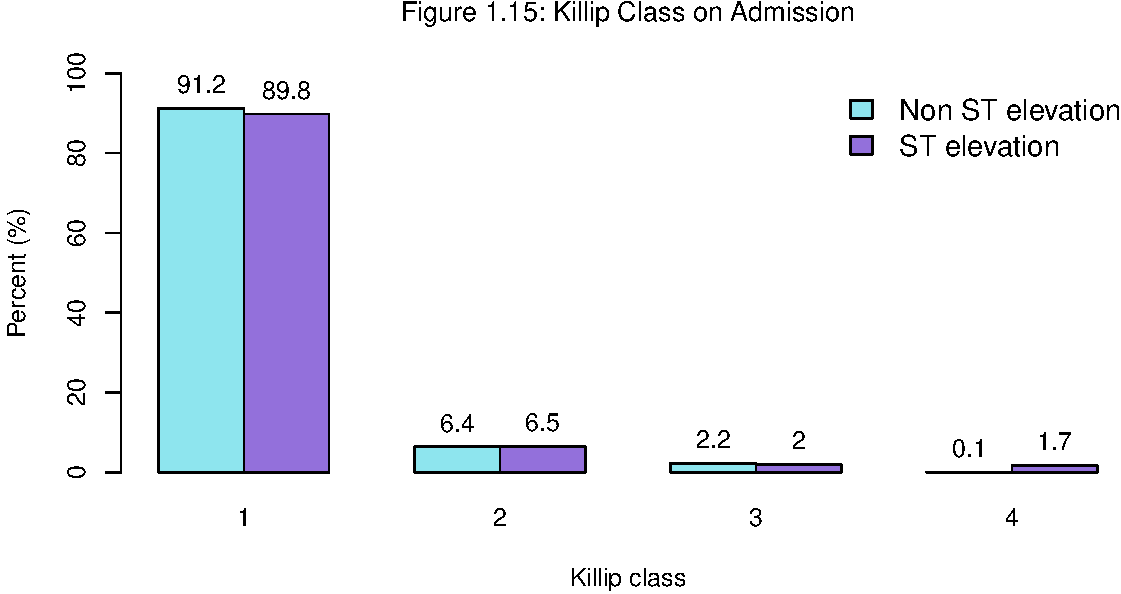
\includegraphics{ACSIS_2024_v1_pdf_files/figure-latex/unnamed-chunk-51-1.pdf}

\pagebreak

\subsubsection{1.5.10 Pre-Hospital Treatment (before ED
arrival)}\label{pre-hospital-treatment-before-ed-arrival}

At first medical contact, patients with ST elevation were significantly
more likely to receive therapy with aspirin and heparin than patients
with non ST elevation.

~

\begin{table}[H]
\centering
\caption{\label{tab:unnamed-chunk-53}Table 1.16 Pre-Hospitalization Treatment}
\centering
\begin{tabular}[t]{>{\raggedright\arraybackslash}p{4cm}>{\centering\arraybackslash}p{3cm}>{\centering\arraybackslash}p{3cm}>{\centering\arraybackslash}p{3cm}>{\centering\arraybackslash}p{1.5cm}}
\toprule
  & Total & Non ST elevation & ST elevation & p-value\\
\midrule
\cellcolor{gray!10}{n\textsuperscript{1}} & \cellcolor{gray!10}{849} & \cellcolor{gray!10}{393} & \cellcolor{gray!10}{454} & \cellcolor{gray!10}{}\\
Aspirin ($\%$) & 492 ( 79.1) & 163 ( 66.8) & 329 ( 87.0) & <0.001\\
\cellcolor{gray!10}{Clopidogrel ($\%$)} & \cellcolor{gray!10}{5 (  0.8)} & \cellcolor{gray!10}{0 (  0.0)} & \cellcolor{gray!10}{5 (  1.3)} & \cellcolor{gray!10}{0.179}\\
Prasugrel ($\%$) & 2 (  0.3) & 0 (  0.0) & 2 (  0.5) & 0.680\\
\cellcolor{gray!10}{Ticagrelor ($\%$)} & \cellcolor{gray!10}{0 (   0.0)} & \cellcolor{gray!10}{0 (   0.0)} & \cellcolor{gray!10}{0 (   0.0)} & \cellcolor{gray!10}{NA}\\
Heparin ($\%$) & 268 ( 43.1) & 24 (  9.8) & 244 ( 64.6) & <0.001\\
\cellcolor{gray!10}{LMWH ($\%$)} & \cellcolor{gray!10}{9 (  1.4)} & \cellcolor{gray!10}{1 (  0.4)} & \cellcolor{gray!10}{8 (  2.1)} & \cellcolor{gray!10}{0.163}\\
\bottomrule
\multicolumn{5}{l}{\rule{0pt}{1em}\textsuperscript{1} Only MICU and regular ambulance patients were included}\\
\end{tabular}
\end{table}

~

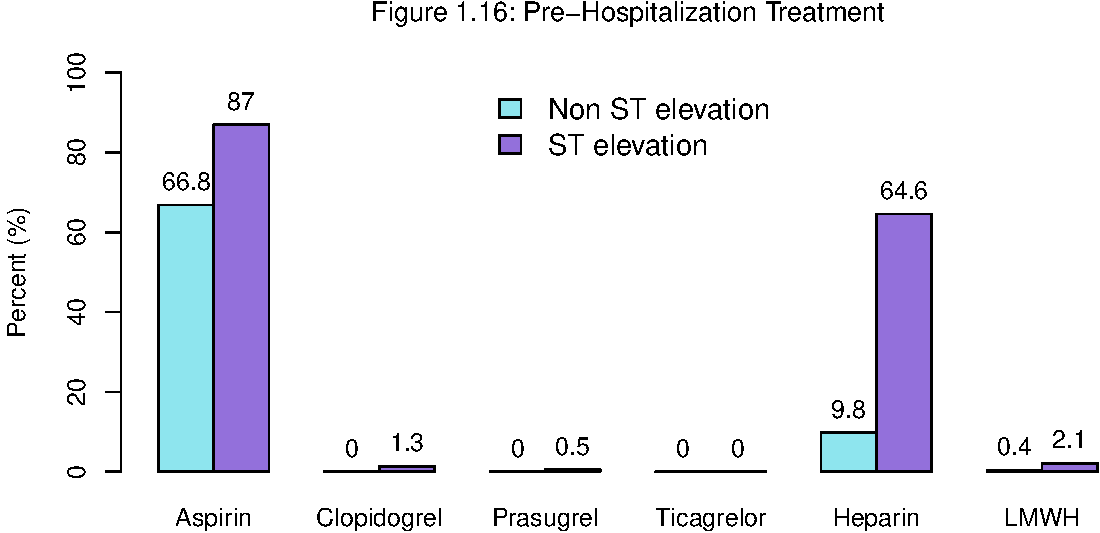
\includegraphics{ACSIS_2024_v1_pdf_files/figure-latex/unnamed-chunk-54-1.pdf}

\pagebreak

\subsection{1.6 First Recorded ECG}\label{first-recorded-ecg}

\subsubsection{1.6.1 Location of First ECG
Recording}\label{location-of-first-ecg-recording}

68.4\% of patients presenting with non ST elevation and 35.2\% of
patients presenting with ST elevation had their first ECG recorded in
the emergency department (ED). With respect to the remaining patients,
46\% of patients with ST elevation and 17.4\% of those with non ST
elevation had the first ECG performed either at home or in an ambulance,
and about 15\% in both groups had it performed in a primary clinic.

~

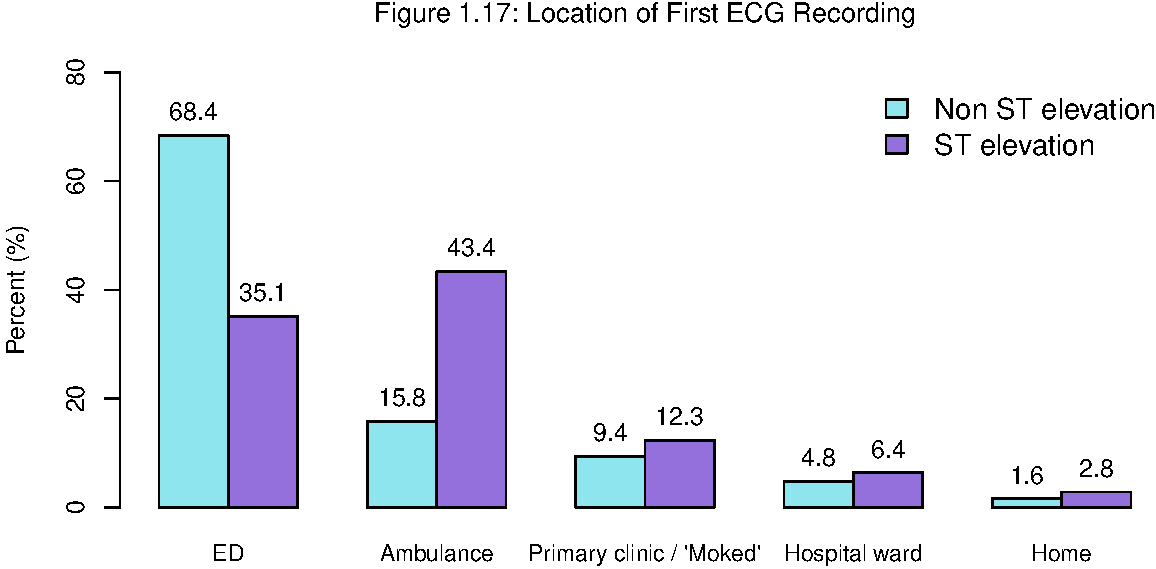
\includegraphics{ACSIS_2024_v1_pdf_files/figure-latex/unnamed-chunk-55-1.pdf}

\pagebreak

\subsubsection{1.6.2 First ECG Rhythm}\label{first-ecg-rhythm}

About 94\% of patients presented with a normal sinus rhythm (NSR). 3.1\%
of patients with ST elevation and 3.9\% of those without ST elevation,
presented with atrial fibrillation.

~

\begin{table}[H]
\centering
\caption{\label{tab:unnamed-chunk-57}Table 1.17: First ECG Rhythm}
\centering
\begin{tabular}[t]{>{\raggedright\arraybackslash}p{5cm}>{\centering\arraybackslash}p{3cm}>{\centering\arraybackslash}p{3cm}>{\centering\arraybackslash}p{3cm}}
\toprule
  & Total & Non ST elevation & ST elevation\\
\midrule
\cellcolor{gray!10}{n} & \cellcolor{gray!10}{1801} & \cellcolor{gray!10}{1085} & \cellcolor{gray!10}{662}\\
NSR (\%) & 1537 (93.7) & 970 (94.4) & 565 (92.3)\\
\cellcolor{gray!10}{Atrial fibrillation (\%)} & \cellcolor{gray!10}{59 ( 3.6)} & \cellcolor{gray!10}{40 ( 3.9)} & \cellcolor{gray!10}{19 ( 3.1)}\\
Ventricular Tachycardia (VT)/ Ventricular Fibrillation (VF) (\%) & 21 ( 1.3) & 7 ( 0.7) & 14 ( 2.3)\\
\cellcolor{gray!10}{High degree (2nd / 3rd) Atrioventricular (AV) Block (\%)} & \cellcolor{gray!10}{14 ( 0.9)} & \cellcolor{gray!10}{5 ( 0.5)} & \cellcolor{gray!10}{9 ( 1.5)}\\
Asystole (\%) & 1 ( 0.1) & 0 ( 0.0) & 1 ( 0.2)\\
\cellcolor{gray!10}{Other (\%)} & \cellcolor{gray!10}{9 ( 0.5)} & \cellcolor{gray!10}{5 ( 0.5)} & \cellcolor{gray!10}{4 ( 0.7)}\\
\bottomrule
\multicolumn{4}{l}{\rule{0pt}{1em}Difference in first ECG rhythm, ST elevation vs. non ST elevation, p  0.011}\\
\end{tabular}
\end{table}

\pagebreak

\subsection{1.7 Primary Reperfusion}\label{primary-reperfusion}

\subsubsection{1.7.1 Primary Reperfusion Therapy in Patients with
STEMI}\label{primary-reperfusion-therapy-in-patients-with-stemi}

88\% of patients with STEMI underwent primary reperfusion within 12
hours from onset of symptoms, mainly primary PCI. In 87.1\% of these
cases, stents were deployed. Of the remaining 12`\% which did not
undergo primary reperfusion, 87.2\% eventually underwent coronary
angiography. Of these, 90\% underwent revascularization.

~

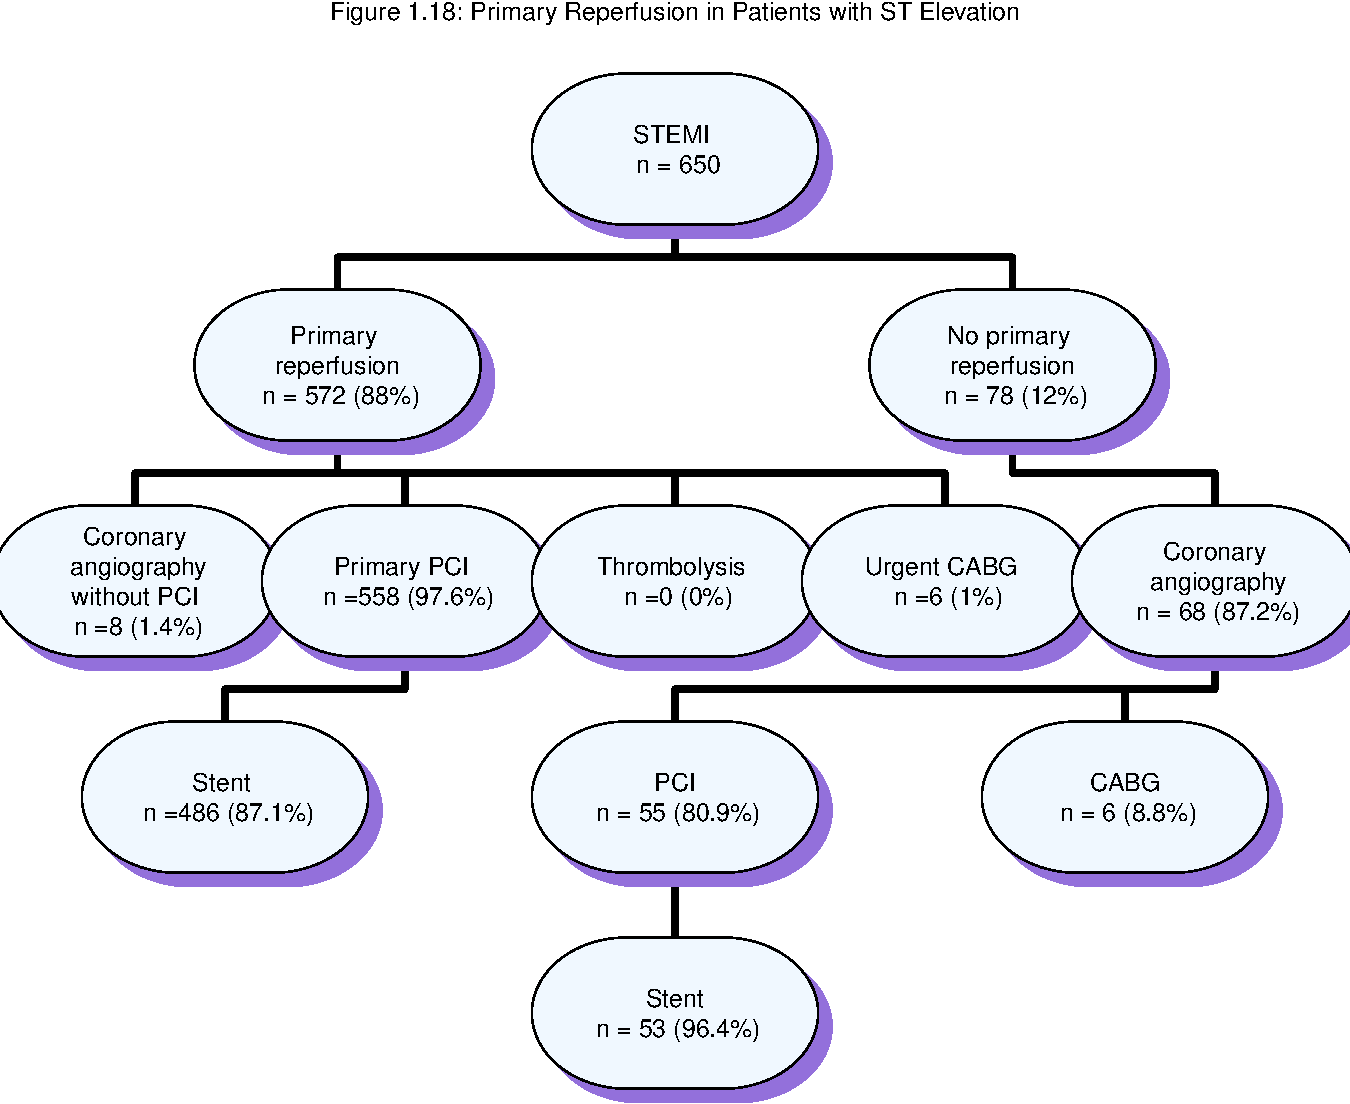
\includegraphics{ACSIS_2024_v1_pdf_files/figure-latex/unnamed-chunk-58-1.pdf}

\pagebreak

\subsubsection{1.7.2 Length of Time from Arrival to Primary
Reperfusion}\label{length-of-time-from-arrival-to-primary-reperfusion}

The median time from arrival to primary reperfusion was less than one
hour (32 minutes).

~

\begin{table}[H]
\centering
\caption{\label{tab:unnamed-chunk-60}Table 1.18: Length of Time (minutes) from Arrival to Reperfusion}
\centering
\begin{tabular}[t]{>{\raggedright\arraybackslash}p{5.9cm}>{\centering\arraybackslash}p{4.3cm}>{\centering\arraybackslash}p{4.3cm}}
\toprule
  & N & Time in minutes (median [IQR])\\
\midrule
\cellcolor{gray!10}{From arrival to  thrombolysis (TLx)} & \cellcolor{gray!10}{0} & \cellcolor{gray!10}{32.00 [14.00, 67.00]}\\
From arrival to primary PCI (PPCI) & 473 & 32.00 [14.00, 67.00]\\
\bottomrule
\end{tabular}
\end{table}

~

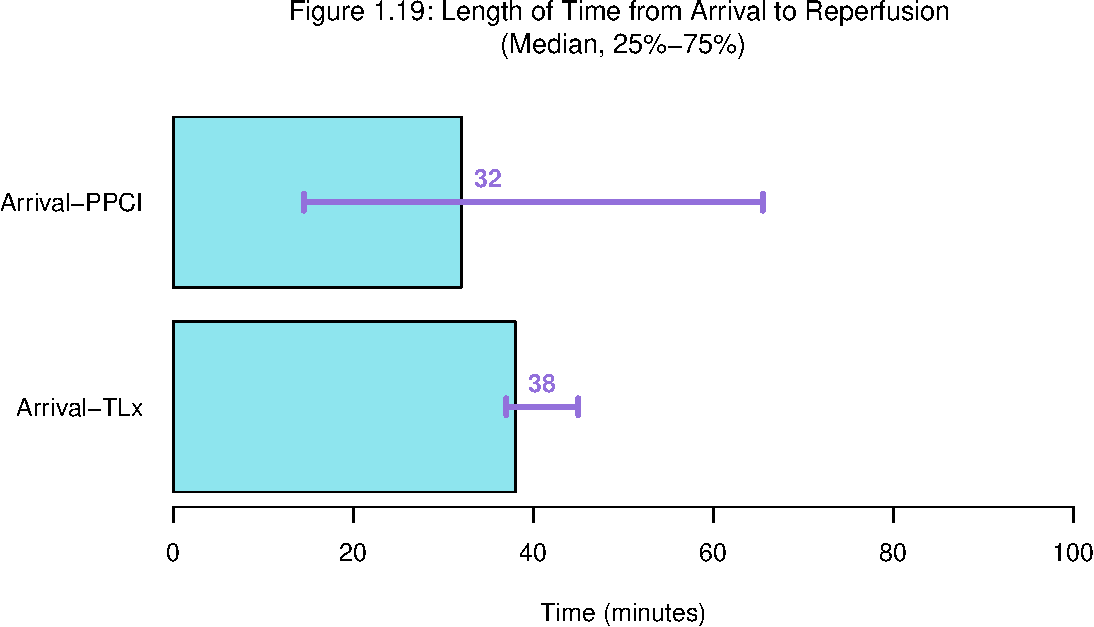
\includegraphics{ACSIS_2024_v1_pdf_files/figure-latex/unnamed-chunk-61-1.pdf}

\pagebreak

\subsubsection{1.7.3 Length of Time from Arrival to Primary Reperfusion,
by
Gender}\label{length-of-time-from-arrival-to-primary-reperfusion-by-gender}

The time delay from arrival to primary reperfusion was shorter for men
compared to women.

~

\begin{table}[H]
\centering
\caption{\label{tab:unnamed-chunk-63}Table 1.19: Length of Time (minutes) from Arrival to Reperfusion, by gender}
\centering
\begin{tabular}[t]{>{\raggedright\arraybackslash}p{4.5cm}>{\centering\arraybackslash}p{3.5cm}>{\centering\arraybackslash}p{1cm}>{\centering\arraybackslash}p{3.5cm}>{\centering\arraybackslash}p{1cm}>{\centering\arraybackslash}p{1cm}}
\toprule
\multicolumn{1}{c}{} & \multicolumn{2}{c}{Women} & \multicolumn{2}{c}{Men} & \multicolumn{1}{c}{} \\
\cmidrule(l{3pt}r{3pt}){2-3} \cmidrule(l{3pt}r{3pt}){4-5}
  & Time in minutes (median [IQR]) & N & Time in minutes (median [IQR]) & N & p-value\\
\midrule
\cellcolor{gray!10}{From arrival to  thrombolysis} & \cellcolor{gray!10}{38  [14.25, 70.75]} & \cellcolor{gray!10}{0} & \cellcolor{gray!10}{42  [16 , 79 ]} & \cellcolor{gray!10}{0} & \cellcolor{gray!10}{0.472}\\
From arrival to primary PCI & 38  [14.25, 70.75] & 90 & 42  [16 , 79 ] & 441 & 0.472\\
\bottomrule
\end{tabular}
\end{table}

~

~

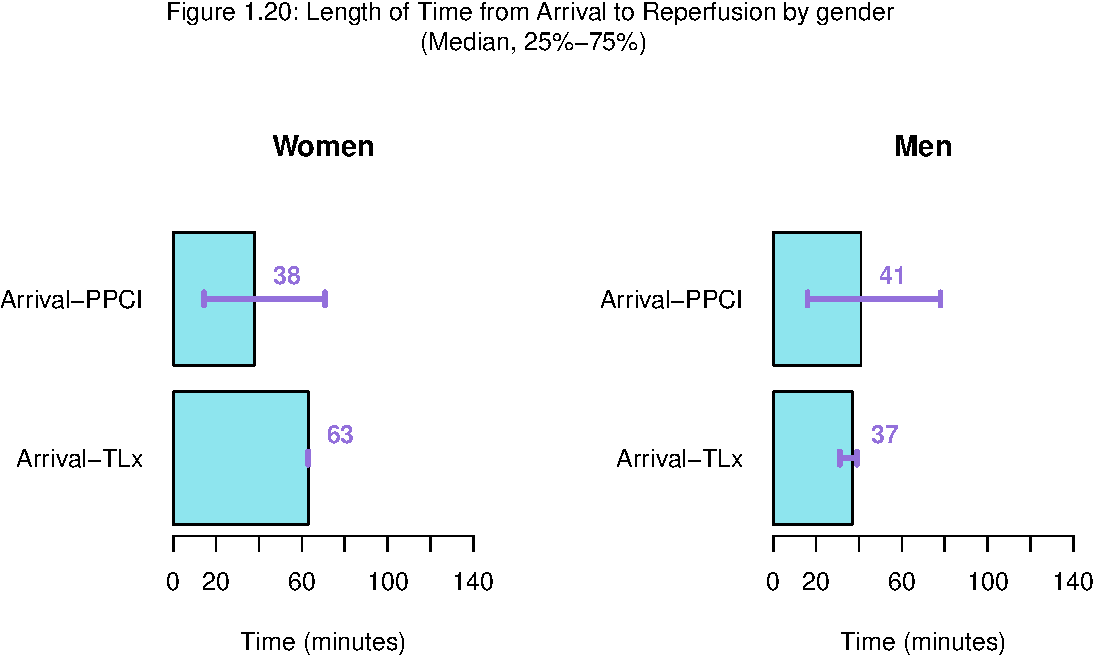
\includegraphics{ACSIS_2024_v1_pdf_files/figure-latex/unnamed-chunk-64-1.pdf}

\pagebreak

\subsubsection{1.7.4 Use of drugs and protective devices during Primary
PCI}\label{use-of-drugs-and-protective-devices-during-primary-pci}

~

\begin{table}[H]
\centering
\caption{\label{tab:unnamed-chunk-66}Table 1.20: Drugs and Protective Devices during Primary Reperfusion}
\centering
\begin{tabular}[t]{>{\raggedright\arraybackslash}p{8cm}>{\centering\arraybackslash}p{6.5cm}}
\toprule
  & Overall\\
\midrule
\cellcolor{gray!10}{n} & \cellcolor{gray!10}{572}\\
IIb/IIIa antagonists (\%) & 142 (24.8)\\
\cellcolor{gray!10}{Bivalirudin (\%)} & \cellcolor{gray!10}{13 ( 2.3)}\\
Aspiration device (\%) & 43 ( 7.5)\\
\bottomrule
\end{tabular}
\end{table}

~

~

\subsubsection{1.7.5 Primary PCI / Coronary
Angiography}\label{primary-pci-coronary-angiography}

\begin{table}[H]
\centering
\caption{\label{tab:unnamed-chunk-68}Table 1.21: Vascular access during Primary Reperfusion}
\centering
\begin{tabular}[t]{>{\raggedright\arraybackslash}p{8cm}>{\centering\arraybackslash}p{6.5cm}}
\toprule
  & Overall\\
\midrule
\cellcolor{gray!10}{n} & \cellcolor{gray!10}{572}\\
Vascular access & \\
\hspace{1em}\cellcolor{gray!10}{Femoral} & \cellcolor{gray!10}{45 ( 8.2)}\\
\hspace{1em}Radial & 497 (91.0)\\
\hspace{1em}\cellcolor{gray!10}{Both} & \cellcolor{gray!10}{4 ( 0.7)}\\
\bottomrule
\end{tabular}
\end{table}

~

~

\subsubsection{1.7.6 Thrombolysis in Myocardial Infarction (TIMI) Grade
Flow of Infarct-Related Artery (IRA) During Primary
PCI}\label{thrombolysis-in-myocardial-infarction-timi-grade-flow-of-infarct-related-artery-ira-during-primary-pci}

In 61\% of cases, a TIMI flow grade of zero was observed on first
injection to the Infarct Related Artery (IRA). Following
revascularization, a TIMI grade flow of 3 was achieved in the majority
of patients (93\%).

~

\begin{table}[H]
\centering
\caption{\label{tab:unnamed-chunk-70}Table 1.22: TIMI Grade Flow of IRA Before and After Revascularization}
\centering
\begin{tabular}[t]{>{\raggedright\arraybackslash}p{5.5cm}>{\centering\arraybackslash}p{5.5cm}>{\centering\arraybackslash}p{5.5cm}}
\toprule
  & Before revascularization ($\%$) & After revascularization ($\%$)\\
\midrule
\cellcolor{gray!10}{n} & \cellcolor{gray!10}{480} & \cellcolor{gray!10}{531}\\
\hspace{2em}0 & 293 (61.0) & 10 ( 1.9)\\
\hspace{2em}\cellcolor{gray!10}{1} & \cellcolor{gray!10}{71 (14.8)} & \cellcolor{gray!10}{3 ( 0.6)}\\
\hspace{2em}2 & 53 (11.0) & 24 ( 4.5)\\
\hspace{2em}\cellcolor{gray!10}{3} & \cellcolor{gray!10}{63 (13.1)} & \cellcolor{gray!10}{494 (93.0)}\\
\bottomrule
\end{tabular}
\end{table}

\pagebreak

\subsubsection{1.7.7 Reasons for Not Performing Primary
Reperfusion}\label{reasons-for-not-performing-primary-reperfusion}

12\% of patients presenting with STEMI did not receive primary
reperfusion therapy. In 21.1\% the reason was spontaneous reperfusion,
in 45.6\% the reason was late arrival at the hospital, and in 21.1\% of
cases primary reperfusion was considered not indicated.

~

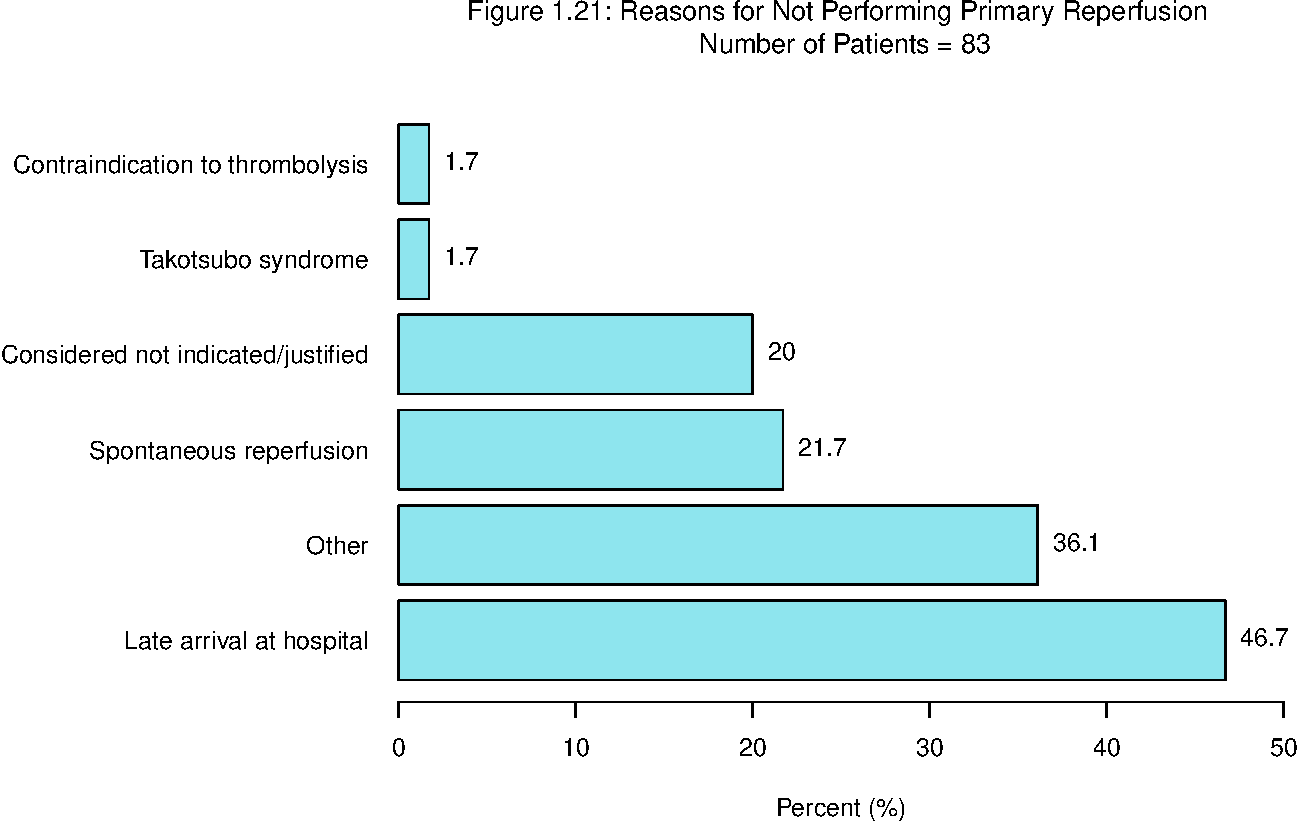
\includegraphics{ACSIS_2024_v1_pdf_files/figure-latex/unnamed-chunk-72-1.pdf}

\begin{itemize}
\tightlist
\item
  There were no patients with contraindication to thrombolysis or
  patient refusal.
\end{itemize}

\pagebreak

\subsection{1.8 Coronary Interventions and Procedures during
Hospitalization}\label{coronary-interventions-and-procedures-during-hospitalization}

\subsubsection{1.8.1 Coronary Angiography and
Interventions}\label{coronary-angiography-and-interventions}

Patients with STEMI were more likely than those with non STEMI to
undergo coronary angiography and PCI. CABG during hospitalization was
performed more frequently in patients with non STEMI.

~

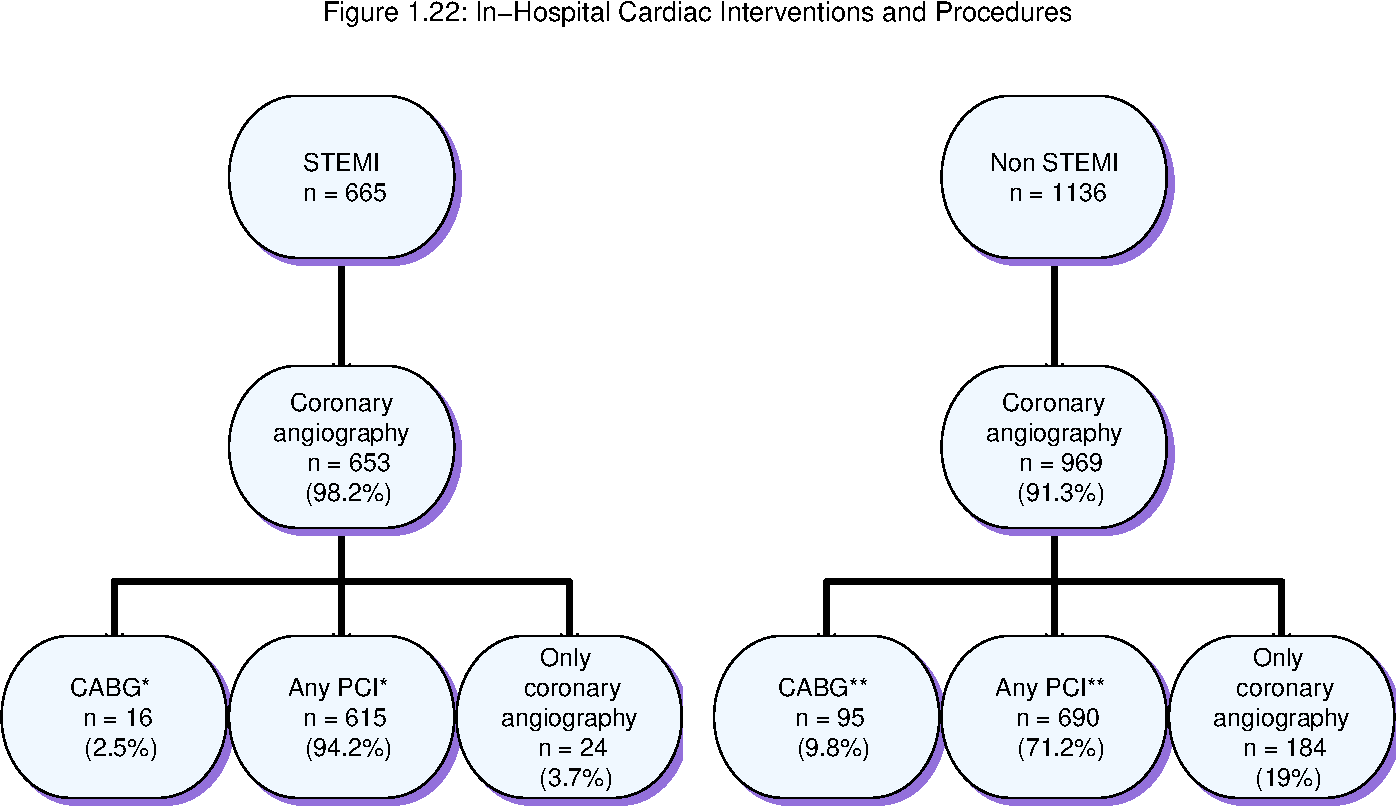
\includegraphics{ACSIS_2024_v1_pdf_files/figure-latex/unnamed-chunk-73-1.pdf}

*2 patients underwent both CABG and PCI;\\
** 2 patients underwent both CABG and PCI.

\pagebreak

\subsubsection{\texorpdfstring{1.8.2 Coronary Angiography
(\textbf{\emph{excluding}} \emph{primary
PCI})}{1.8.2 Coronary Angiography (excluding primary PCI)}}\label{coronary-angiography-excluding-primary-pci}

\begin{table}[H]
\centering
\caption{\label{tab:unnamed-chunk-75}Table 1.23: Vascular access during coronary angiography}
\centering
\begin{tabular}[t]{>{\raggedright\arraybackslash}p{8cm}>{\centering\arraybackslash}p{6.5cm}}
\toprule
  & Overall\\
\midrule
\cellcolor{gray!10}{n} & \cellcolor{gray!10}{1201}\\
Coronary angiography & 1030 (89.6)\\
\hspace{1em}\cellcolor{gray!10}{Vascular access:} & \cellcolor{gray!10}{}\\
\hspace{1em}\hspace{1em}Femoral & 50 ( 5.0)\\
\hspace{1em}\hspace{1em}\cellcolor{gray!10}{Radial} & \cellcolor{gray!10}{935 (94.3)}\\
\addlinespace
\hspace{1em}\hspace{1em}Both & 6 ( 0.6)\\
\bottomrule
\end{tabular}
\end{table}

~

~

\subsubsection{1.8.3 Other Procedures During
Hospitalization}\label{other-procedures-during-hospitalization}

Patients with STEMI were more likely to receive Direct-Current (DC)
shocks, resuscitation and therapeutic hypothermia than those with non
STEMI.

~

\begin{table}[H]
\centering
\caption{\label{tab:unnamed-chunk-78}Table 1.24: Other Procedures}
\centering
\begin{tabular}[t]{>{\raggedright\arraybackslash}p{5.2cm}>{\centering\arraybackslash}p{2.5cm}>{\centering\arraybackslash}p{2.5cm}>{\centering\arraybackslash}p{2.5cm}>{\centering\arraybackslash}p{1.5cm}}
\toprule
  & Total & Non STEMI & STEMI & p-value\\
\midrule
\cellcolor{gray!10}{n} & \cellcolor{gray!10}{1801} & \cellcolor{gray!10}{1151} & \cellcolor{gray!10}{650} & \cellcolor{gray!10}{}\\
DC shock (\%) & 54 ( 3.1) & 18 ( 1.6) & 36 ( 5.6) & <0.001\\
\cellcolor{gray!10}{Resuscitation (\%)} & \cellcolor{gray!10}{39 ( 2.2)} & \cellcolor{gray!10}{13 ( 1.2)} & \cellcolor{gray!10}{26 ( 4.0)} & \cellcolor{gray!10}{<0.001}\\
Mechanical ventilation (\%) &  &  &  & 0.016\\
\hspace{1em}\cellcolor{gray!10}{Invasive} & \cellcolor{gray!10}{48 ( 2.8)} & \cellcolor{gray!10}{21 ( 1.9)} & \cellcolor{gray!10}{27 ( 4.2)} & \cellcolor{gray!10}{}\\
\hspace{1em}Non invasive & 41 ( 2.4) & 24 ( 2.2) & 17 ( 2.6) & \\
\cellcolor{gray!10}{Intra-Aortic Balloon Pump (IABP) (\%)} & \cellcolor{gray!10}{18 ( 1.1)} & \cellcolor{gray!10}{4 ( 0.4)} & \cellcolor{gray!10}{14 ( 2.3)} & \cellcolor{gray!10}{0.001}\\
Dialysis (\%) & 9 ( 0.5) & 8 ( 0.7) & 1 ( 0.2) & 0.204\\
\cellcolor{gray!10}{ICD/CRT (\%)} & \cellcolor{gray!10}{13 ( 0.7)} & \cellcolor{gray!10}{8 ( 0.7)} & \cellcolor{gray!10}{5 ( 0.8)} & \cellcolor{gray!10}{1.000}\\
Permanent pacemaker (\%) & 10 ( 0.6) & 8 ( 0.7) & 2 ( 0.3) & 0.424\\
\cellcolor{gray!10}{Temporary pacemaker (\%)} & \cellcolor{gray!10}{14 ( 0.8)} & \cellcolor{gray!10}{3 ( 0.3)} & \cellcolor{gray!10}{11 ( 1.7)} & \cellcolor{gray!10}{0.003}\\
Temperature control (\%) & 3 ( 0.2) & 0 ( 0.0) & 3 ( 0.5) & 0.096\\
\bottomrule
\end{tabular}
\end{table}

\pagebreak

\subsection{1.9 Ejection Fraction}\label{ejection-fraction}

Ejection fraction (EF) was determined in 98.6\% of patients with STEMI
and in 91.2\% of those with non STEMI. EF was normal in a larger
proportion of patients with non STEMI (50.7\%) than in patients with
STEMI (20.7\%). 29.9\% of patients with STEMI and 15.1\% of patients
with non STEMI presented with an EF \textless{} 40\%.

~

\begin{table}[H]
\centering
\caption{\label{tab:unnamed-chunk-80}Table 1.25: Ejection Fraction}
\centering
\begin{tabular}[t]{>{\raggedright\arraybackslash}p{4.9cm}>{\centering\arraybackslash}p{2.7cm}>{\centering\arraybackslash}p{2.7cm}>{\centering\arraybackslash}p{2.7cm}>{\centering\arraybackslash}p{1.5cm}}
\toprule
  & Total & Non STEMI & STEMI & p-value\\
\midrule
\cellcolor{gray!10}{n} & \cellcolor{gray!10}{1801} & \cellcolor{gray!10}{1151} & \cellcolor{gray!10}{650} & \cellcolor{gray!10}{}\\
EF determined ($\%$) & 1568 (93.9) & 948 (91.2) & 620 (98.6) & <0.001\\
\hspace{0.6em}\cellcolor{gray!10}{EF (range) ($\%$)} & \cellcolor{gray!10}{} & \cellcolor{gray!10}{} & \cellcolor{gray!10}{} & \cellcolor{gray!10}{<0.001}\\
\hspace{1.2em}Normal (55-65$\%$) & 608 (38.9) & 480 (50.7) & 128 (20.7) & \\
\hspace{1.2em}\cellcolor{gray!10}{Preserved (50-54$\%$)} & \cellcolor{gray!10}{192 (12.3)} & \cellcolor{gray!10}{114 (12.0)} & \cellcolor{gray!10}{78 (12.6)} & \cellcolor{gray!10}{}\\
\hspace{1.2em}Mild (40-49$\%$) & 436 (27.9) & 210 (22.2) & 226 (36.6) & \\
\hspace{1.2em}\cellcolor{gray!10}{Moderate (30-39$\%$)} & \cellcolor{gray!10}{236 (15.1)} & \cellcolor{gray!10}{100 (10.6)} & \cellcolor{gray!10}{136 (22.0)} & \cellcolor{gray!10}{}\\
\hspace{1.2em}Severe (< 30$\%$) & 92 ( 5.9) & 43 ( 4.5) & 49 ( 7.9) & \\
\bottomrule
\multicolumn{5}{l}{\rule{0pt}{1em}\textit{Note: }}\\
\multicolumn{5}{l}{\rule{0pt}{1em}EF range percentages are calculated out of patients who had documented EF}\\
\end{tabular}
\end{table}

\pagebreak

\subsection{1.10 In-Hospital
Complications}\label{in-hospital-complications}

Cardiogenic shock, CHF mild-moderate, hemodynamically significant Right
Ventricular (RV) infarction, ventricular fibrillation (VF), new Atrial
fibrillation (AF) and high degree (2nd / 3rd) Atrioventricular Block
(AVB) were more frequent in patients with STEMI.

~

\begin{table}[H]
\centering
\caption{\label{tab:unnamed-chunk-82}Table 1.26: In-Hospital Complications}
\centering
\begin{tabular}[t]{>{\raggedright\arraybackslash}p{8cm}>{\centering\arraybackslash}p{1.7cm}>{\centering\arraybackslash}p{1.7cm}>{\centering\arraybackslash}p{1.7cm}>{\centering\arraybackslash}p{1.4cm}}
\toprule
  & Total & Non STEMI & STEMI & p-value\\
\midrule
\cellcolor{gray!10}{n} & \cellcolor{gray!10}{1801} & \cellcolor{gray!10}{1151} & \cellcolor{gray!10}{650} & \cellcolor{gray!10}{}\\
CHF mild-moderate (Killip-2) (\%) & 179 (10.3) & 90 (8.2) & 89 (13.8) & <0.001\\
\cellcolor{gray!10}{Pulmonary edema (Killip-3) (\%)} & \cellcolor{gray!10}{59 ( 3.4)} & \cellcolor{gray!10}{33 (3.0)} & \cellcolor{gray!10}{26 ( 4.0)} & \cellcolor{gray!10}{0.326}\\
Cardiogenic shock (Killip-4) (\%) & 41 ( 2.4) & 11 (1.0) & 30 ( 4.6) & <0.001\\
\cellcolor{gray!10}{Hemodynamically significant RV infarction (\%)} & \cellcolor{gray!10}{7 ( 0.4)} & \cellcolor{gray!10}{3 (0.3)} & \cellcolor{gray!10}{4 ( 0.6)} & \cellcolor{gray!10}{0.481}\\
Re-MI (\%) & 10 ( 0.6) & 7 (0.6) & 3 ( 0.5) & 0.890\\
\cellcolor{gray!10}{Post MI angina/re-ischemia (\%)} & \cellcolor{gray!10}{19 ( 1.1)} & \cellcolor{gray!10}{13 (1.2)} & \cellcolor{gray!10}{6 ( 0.9)} & \cellcolor{gray!10}{0.791}\\
Stent thrombosis (definite/probable/possible) (\%) & 11 ( 0.6) & 3 (0.3) & 8 ( 1.2) & 0.033\\
\cellcolor{gray!10}{Free wall rupture (\%)} & \cellcolor{gray!10}{3 ( 0.2)} & \cellcolor{gray!10}{1 (0.1)} & \cellcolor{gray!10}{2 ( 0.3)} & \cellcolor{gray!10}{0.645}\\
Tamponade (\%) & 1 ( 0.1) & 1 (0.1) & 0 ( 0.0) & 1.000\\
\cellcolor{gray!10}{MR Moderate-severe (\%)} & \cellcolor{gray!10}{25 ( 1.4)} & \cellcolor{gray!10}{11 (1.0)} & \cellcolor{gray!10}{14 ( 2.2)} & \cellcolor{gray!10}{0.079}\\
Pericarditis (\%) & 12 ( 0.7) & 5 (0.5) & 7 ( 1.1) & 0.222\\
\cellcolor{gray!10}{Sustained VT (>125 bpm) (\%)} & \cellcolor{gray!10}{16 ( 0.9)} & \cellcolor{gray!10}{8 (0.7)} & \cellcolor{gray!10}{8 ( 1.2)} & \cellcolor{gray!10}{0.418}\\
VF (\%) & 33 ( 1.9) & 7 (0.6) & 26 ( 4.0) & <0.001\\
\cellcolor{gray!10}{New AF (\%)} & \cellcolor{gray!10}{57 ( 3.3)} & \cellcolor{gray!10}{35 (3.2)} & \cellcolor{gray!10}{22 ( 3.4)} & \cellcolor{gray!10}{0.932}\\
High degree (2nd / 3rd) AVB (\%) & 22 ( 1.3) & 10 (0.9) & 12 ( 1.8) & 0.140\\
\cellcolor{gray!10}{Asystole (\%)} & \cellcolor{gray!10}{13 ( 0.7)} & \cellcolor{gray!10}{7 (0.6)} & \cellcolor{gray!10}{6 ( 0.9)} & \cellcolor{gray!10}{0.700}\\
TIA (\%) & 4 ( 0.2) & 3 (0.3) & 1 ( 0.2) & 1.000\\
\cellcolor{gray!10}{Stroke (\%)} & \cellcolor{gray!10}{5 ( 0.3)} & \cellcolor{gray!10}{2 (0.2)} & \cellcolor{gray!10}{3 ( 0.5)} & \cellcolor{gray!10}{0.551}\\
CVA/TIA in hospital (\%) & 9 ( 0.5) & 5 (0.4) & 4 ( 0.6) & 0.861\\
\cellcolor{gray!10}{Acute renal injury (\%)} & \cellcolor{gray!10}{71 ( 4.3)} & \cellcolor{gray!10}{46 (4.5)} & \cellcolor{gray!10}{25 ( 4.0)} & \cellcolor{gray!10}{0.707}\\
Sepsis (\%) & 24 ( 1.5) & 13 (1.3) & 11 ( 1.8) & 0.566\\
\cellcolor{gray!10}{Bleeding (\%)} & \cellcolor{gray!10}{11 ( 0.7)} & \cellcolor{gray!10}{7 (0.7)} & \cellcolor{gray!10}{4 ( 0.6)} & \cellcolor{gray!10}{1.000}\\
Minor bleeding (\%) & 9 ( 0.6) & 5 (0.5) & 4 ( 0.6) & 0.965\\
\cellcolor{gray!10}{Blood transfusions (\%)} & \cellcolor{gray!10}{6 ( 0.4)} & \cellcolor{gray!10}{5 (0.5)} & \cellcolor{gray!10}{1 ( 0.2)} & \cellcolor{gray!10}{0.506}\\
\bottomrule
\end{tabular}
\end{table}

\pagebreak

\subsection{1.11 In-Hospital Medical
Treatment}\label{in-hospital-medical-treatment}

Aspirin, prasugrel, P2Y12 inhibitors, ACE-I/ARB, Spironolactone,
beta-blockers, Proton-Pump Inhibitors (PPI), IV inotropic agent and
statins were more frequently used in patients with STEMI. Clopidogrel,
CCB and nitrates were more frequently used among patients with non
STEMI.

All other recommended drugs were similarly given to both groups.

\begin{table}[H]
\centering
\caption{\label{tab:unnamed-chunk-84}Table 1.27: In-Hospital Medical Treatment}
\centering
\fontsize{9.5}{11.5}\selectfont
\begin{tabular}[t]{>{\raggedright\arraybackslash}p{6cm}>{\centering\arraybackslash}p{2.5cm}>{\centering\arraybackslash}p{2.5cm}>{\centering\arraybackslash}p{2.5cm}>{\centering\arraybackslash}p{1cm}}
\toprule
  & Total & Non STEMI & STEMI & p-value\\
\midrule
\cellcolor{gray!10}{n} & \cellcolor{gray!10}{1801} & \cellcolor{gray!10}{1151} & \cellcolor{gray!10}{650} & \cellcolor{gray!10}{}\\
\addlinespace[0.3em]
\multicolumn{5}{l}{\textbf{Anti-platelets}}\\
\hspace{1em}Aspirin ($\%$) & 1384 ( 76.8) & 840 ( 73.0) & 544 ( 83.7) & <0.001\\
\hspace{1em}\cellcolor{gray!10}{P2Y12 inhibitors ($\%$)} & \cellcolor{gray!10}{1212 ( 67.3)} & \cellcolor{gray!10}{692 ( 60.1)} & \cellcolor{gray!10}{520 ( 80.0)} & \cellcolor{gray!10}{<0.001}\\
\hspace{1em}Clopidogrel ($\%$) & 386 ( 21.4) & 297 ( 25.8) & 89 ( 13.7) & <0.001\\
\hspace{1em}\cellcolor{gray!10}{Prasugrel ($\%$)} & \cellcolor{gray!10}{479 ( 26.6)} & \cellcolor{gray!10}{184 ( 16.0)} & \cellcolor{gray!10}{295 ( 45.4)} & \cellcolor{gray!10}{<0.001}\\
\hspace{1em}Ticagrelor ($\%$) & 380 ( 21.1) & 224 ( 19.5) & 156 ( 24.0) & 0.027\\
\addlinespace[0.3em]
\multicolumn{5}{l}{\textbf{Anticoagulants}}\\
\hspace{1em}\cellcolor{gray!10}{Oral anticoagulants\textsuperscript{1} ($\%$)} & \cellcolor{gray!10}{107 (  5.9)} & \cellcolor{gray!10}{57 (  5.0)} & \cellcolor{gray!10}{50 (  7.7)} & \cellcolor{gray!10}{0.024}\\
\hspace{1em}Warfarin ($\%$) & 22 (  1.2) & 12 (  1.0) & 10 (  1.5) & 0.486\\
\hspace{1em}\cellcolor{gray!10}{Dabigatran ($\%$)} & \cellcolor{gray!10}{0 (   0.0)} & \cellcolor{gray!10}{0 (   0.0)} & \cellcolor{gray!10}{0 (   0.0)} & \cellcolor{gray!10}{NA}\\
\hspace{1em}Rivaroxaban ($\%$) & 9 (  0.5) & 4 (  0.3) & 5 (  0.8) & 0.384\\
\hspace{1em}\cellcolor{gray!10}{Apixaban ($\%$)} & \cellcolor{gray!10}{80 (  4.4)} & \cellcolor{gray!10}{44 (  3.8)} & \cellcolor{gray!10}{36 (  5.5)} & \cellcolor{gray!10}{0.115}\\
\addlinespace[0.3em]
\multicolumn{5}{l}{\textbf{Other}}\\
\hspace{1em}ACE-I ($\%$) & 836 ( 76.7) & 699 ( 74.6) & 137 ( 89.5) & <0.001\\
\hspace{1em}\cellcolor{gray!10}{ARB ($\%$)} & \cellcolor{gray!10}{34 (  3.1)} & \cellcolor{gray!10}{31 (  3.3)} & \cellcolor{gray!10}{3 (  1.9)} & \cellcolor{gray!10}{0.527}\\
\hspace{1em}Spironolactone ($\%$) & 214 ( 11.9) & 137 ( 11.9) & 77 ( 11.8) & 1.000\\
\hspace{1em}\cellcolor{gray!10}{Beta Blockers ($\%$)} & \cellcolor{gray!10}{766 ( 42.5)} & \cellcolor{gray!10}{404 ( 35.1)} & \cellcolor{gray!10}{362 ( 55.7)} & \cellcolor{gray!10}{<0.001}\\
\hspace{1em}Digoxin ($\%$) & 223 ( 12.4) & 99 (  8.6) & 124 ( 19.1) & <0.001\\
\hspace{1em}\cellcolor{gray!10}{CCB ($\%$)} & \cellcolor{gray!10}{777 ( 43.1)} & \cellcolor{gray!10}{408 ( 35.4)} & \cellcolor{gray!10}{369 ( 56.8)} & \cellcolor{gray!10}{<0.001}\\
\hspace{1em}Amiodarone ($\%$) & 5 (  0.3) & 2 (  0.2) & 3 (  0.5) & 0.517\\
\hspace{1em}\cellcolor{gray!10}{Other Anti-Arrhythmic ($\%$)} & \cellcolor{gray!10}{143 (  7.9)} & \cellcolor{gray!10}{100 (  8.7)} & \cellcolor{gray!10}{43 (  6.6)} & \cellcolor{gray!10}{0.141}\\
\hspace{1em}Nitrates ($\%$) & 51 (  2.8) & 28 (  2.4) & 23 (  3.5) & 0.226\\
\hspace{1em}\cellcolor{gray!10}{Diuretics ($\%$)} & \cellcolor{gray!10}{6 (  0.3)} & \cellcolor{gray!10}{2 (  0.2)} & \cellcolor{gray!10}{4 (  0.6)} & \cellcolor{gray!10}{0.256}\\
\hspace{1em}Proton-Pump Inhibitors (PPI) ($\%$) & 78 (  4.3) & 55 (  4.8) & 23 (  3.5) & 0.262\\
\hspace{1em}\cellcolor{gray!10}{H2 Blockers ($\%$)} & \cellcolor{gray!10}{184 ( 10.2)} & \cellcolor{gray!10}{116 ( 10.1)} & \cellcolor{gray!10}{68 ( 10.5)} & \cellcolor{gray!10}{0.860}\\
\hspace{1em}NSAIDS ($\%$) & 791 ( 43.9) & 440 ( 38.2) & 351 ( 54.0) & <0.001\\
\hspace{1em}\cellcolor{gray!10}{Colchicine ($\%$)} & \cellcolor{gray!10}{20 (  1.1)} & \cellcolor{gray!10}{15 (  1.3)} & \cellcolor{gray!10}{5 (  0.8)} & \cellcolor{gray!10}{0.421}\\
\hspace{1em}Steroids ($\%$) & 29 (  1.6) & 19 (  1.7) & 10 (  1.5) & 1.000\\
\hspace{1em}\cellcolor{gray!10}{IV inotropic agent ($\%$)} & \cellcolor{gray!10}{3 (  0.9)} & \cellcolor{gray!10}{1 (  0.4)} & \cellcolor{gray!10}{2 (  1.7)} & \cellcolor{gray!10}{0.568}\\
\hspace{1em}Antihyperglycemic\textsuperscript{2} ($\%$) & 175 ( 22.5) & 96 ( 18.0) & 79 ( 32.1) & <0.001\\
\hspace{1em}\cellcolor{gray!10}{Statins ($\%$)} & \cellcolor{gray!10}{1007 ( 55.9)} & \cellcolor{gray!10}{565 ( 49.1)} & \cellcolor{gray!10}{442 ( 68.0)} & \cellcolor{gray!10}{<0.001}\\
\hspace{1em}Ezetimibe ($\%$) & 367 ( 20.4) & 189 ( 16.4) & 178 ( 27.4) & <0.001\\
\bottomrule
\multicolumn{5}{l}{\rule{0pt}{1em}\textsuperscript{1} Oral anticoagulants include warfarin, dabigatran, rivaroxaban and apixaban}\\
\multicolumn{5}{l}{\rule{0pt}{1em}\textsuperscript{2} Only among diabetic patients}\\
\end{tabular}
\end{table}

\pagebreak

\subsection{1.12 Duration of
Hospitalization}\label{duration-of-hospitalization}

~

\begin{table}[H]
\centering
\caption{\label{tab:unnamed-chunk-86}Table 1.28: Length of Stay in ICCU/Cardiology and Total Hospital Stay}
\centering
\begin{tabular}[t]{>{\raggedright\arraybackslash}p{8cm}>{\centering\arraybackslash}p{2cm}>{\centering\arraybackslash}p{2cm}>{\centering\arraybackslash}p{2cm}}
\toprule
  & Total & Non STEMI & STEMI\\
\midrule
\cellcolor{gray!10}{n} & \cellcolor{gray!10}{1801} & \cellcolor{gray!10}{1151} & \cellcolor{gray!10}{650}\\
No. of days in ICCU/Cardiology (median [IQR]) & 3  [2 , 4 ] & 3  [2 , 4 ] & 3  [3 , 5 ]\\
\cellcolor{gray!10}{Total hospital days (median [IQR])} & \cellcolor{gray!10}{3  [2 , 4 ]} & \cellcolor{gray!10}{3  [2 , 4 ]} & \cellcolor{gray!10}{3  [3 , 5 ]}\\
\bottomrule
\end{tabular}
\end{table}

\pagebreak

\subsection{1.13 Discharge}\label{discharge}

\subsection{1.13.1 Medical Treatment on
Discharge}\label{medical-treatment-on-discharge}

Aspirin, P2Y12 inhibitors (mainly prasugrel), ACE-I/ARB, Spironolactone,
beta-blockers and statins were more often prescribed for patients with
STEMI.\\
Clopidogrel, oral anticoagulants, apixaban, CCB, nitrates, and diuretics
were prescribed more often for patients with non STEMI. All other
recommended drugs were similarly given to both groups.

~

\begin{table}[H]
\centering
\caption{\label{tab:unnamed-chunk-88}Table 1.29.a: Medical Treatment on Discharge among Hospital Survivors}
\centering
\begin{tabular}[t]{>{\raggedright\arraybackslash}p{5.8cm}>{\centering\arraybackslash}p{2.5cm}>{\centering\arraybackslash}p{2.5cm}>{\centering\arraybackslash}p{2.5cm}>{\centering\arraybackslash}p{1.2cm}}
\toprule
  & Total & Non STEMI & STEMI & p-value\\
\midrule
\cellcolor{gray!10}{n} & \cellcolor{gray!10}{1720} & \cellcolor{gray!10}{1084} & \cellcolor{gray!10}{636} & \cellcolor{gray!10}{}\\
\addlinespace[0.3em]
\multicolumn{5}{l}{\textbf{Anti-platelets}}\\
\hspace{1em}Aspirin ($\%$) & 1320 ( 76.7) & 806 ( 74.4) & 514 ( 80.8) & 0.003\\
\hspace{1em}\cellcolor{gray!10}{P2Y12 inhibitors ($\%$)} & \cellcolor{gray!10}{1271 ( 73.9)} & \cellcolor{gray!10}{748 ( 69.0)} & \cellcolor{gray!10}{523 ( 82.2)} & \cellcolor{gray!10}{<0.001}\\
\hspace{1em}Clopidogrel ($\%$) & 392 ( 22.8) & 315 ( 29.1) & 77 ( 12.1) & <0.001\\
\hspace{1em}\cellcolor{gray!10}{Prasugrel ($\%$)} & \cellcolor{gray!10}{500 ( 29.1)} & \cellcolor{gray!10}{203 ( 18.7)} & \cellcolor{gray!10}{297 ( 46.7)} & \cellcolor{gray!10}{<0.001}\\
\hspace{1em}Ticagrelor ($\%$) & 379 ( 22.0) & 230 ( 21.2) & 149 ( 23.4) & 0.314\\
\addlinespace[0.3em]
\multicolumn{5}{l}{\textbf{Anticoagulants}}\\
\hspace{1em}\cellcolor{gray!10}{Oral anticoagulants\textsuperscript{1} ($\%$)} & \cellcolor{gray!10}{129 (  7.5)} & \cellcolor{gray!10}{84 (  7.7)} & \cellcolor{gray!10}{45 (  7.1)} & \cellcolor{gray!10}{0.677}\\
\hspace{1em}Warfarin ($\%$) & 8 (  0.5) & 6 (  0.6) & 2 (  0.3) & 0.737\\
\hspace{1em}\cellcolor{gray!10}{Dabigatran ($\%$)} & \cellcolor{gray!10}{0 (   0.0)} & \cellcolor{gray!10}{0 (   0.0)} & \cellcolor{gray!10}{0 (   0.0)} & \cellcolor{gray!10}{NA}\\
\hspace{1em}Rivaroxaban ($\%$) & 11 (  0.6) & 7 (  0.6) & 4 (  0.6) & 1.000\\
\hspace{1em}\cellcolor{gray!10}{Apixaban ($\%$)} & \cellcolor{gray!10}{110 (  6.4)} & \cellcolor{gray!10}{71 (  6.5)} & \cellcolor{gray!10}{39 (  6.1)} & \cellcolor{gray!10}{0.811}\\
\addlinespace[0.3em]
\multicolumn{5}{l}{\textbf{Other}}\\
\hspace{1em}ACE-I ($\%$) & 739 ( 43.0) & 408 ( 37.6) & 331 ( 52.0) & <0.001\\
\hspace{1em}\cellcolor{gray!10}{ARB ($\%$)} & \cellcolor{gray!10}{339 ( 19.7)} & \cellcolor{gray!10}{228 ( 21.0)} & \cellcolor{gray!10}{111 ( 17.5)} & \cellcolor{gray!10}{0.082}\\
\hspace{1em}Spironolactone ($\%$) & 253 ( 14.7) & 121 ( 11.2) & 132 ( 20.8) & <0.001\\
\hspace{1em}\cellcolor{gray!10}{Beta Blockers ($\%$)} & \cellcolor{gray!10}{1052 ( 61.2)} & \cellcolor{gray!10}{615 ( 56.7)} & \cellcolor{gray!10}{437 ( 68.7)} & \cellcolor{gray!10}{<0.001}\\
\hspace{1em}Digoxin ($\%$) & 5 (  0.3) & 2 (  0.2) & 3 (  0.5) & 0.546\\
\hspace{1em}\cellcolor{gray!10}{CCB ($\%$)} & \cellcolor{gray!10}{251 ( 14.6)} & \cellcolor{gray!10}{190 ( 17.5)} & \cellcolor{gray!10}{61 (  9.6)} & \cellcolor{gray!10}{<0.001}\\
\hspace{1em}Amiodarone ($\%$) & 52 (  3.0) & 35 (  3.2) & 17 (  2.7) & 0.614\\
\hspace{1em}\cellcolor{gray!10}{Other Anti-Arrhythmic ($\%$)} & \cellcolor{gray!10}{6 (  0.3)} & \cellcolor{gray!10}{3 (  0.3)} & \cellcolor{gray!10}{3 (  0.5)} & \cellcolor{gray!10}{0.812}\\
\hspace{1em}Nitrates ($\%$) & 46 (  2.7) & 40 (  3.7) & 6 (  0.9) & 0.001\\
\hspace{1em}\cellcolor{gray!10}{Diuretics ($\%$)} & \cellcolor{gray!10}{227 ( 13.2)} & \cellcolor{gray!10}{161 ( 14.9)} & \cellcolor{gray!10}{66 ( 10.4)} & \cellcolor{gray!10}{0.010}\\
\hspace{1em}PPI ($\%$) & 1019 ( 59.2) & 614 ( 56.6) & 405 ( 63.7) & 0.005\\
\hspace{1em}\cellcolor{gray!10}{H2 Blockers ($\%$)} & \cellcolor{gray!10}{23 (  1.3)} & \cellcolor{gray!10}{18 (  1.7)} & \cellcolor{gray!10}{5 (  0.8)} & \cellcolor{gray!10}{0.191}\\
\hspace{1em}Colchicine ($\%$) & 34 (  2.0) & 19 (  1.8) & 15 (  2.4) & 0.489\\
\hspace{1em}\cellcolor{gray!10}{Steroids ($\%$)} & \cellcolor{gray!10}{4 (  1.2)} & \cellcolor{gray!10}{2 (  0.9)} & \cellcolor{gray!10}{2 (  1.8)} & \cellcolor{gray!10}{0.904}\\
\hspace{1em}Antihyperglycemic\textsuperscript{2} ($\%$) & 309 ( 40.2) & 197 ( 37.3) & 112 ( 46.7) & 0.018\\
\hspace{1em}\cellcolor{gray!10}{Glucagon-Like Peptide-1 receptor agonists (GLP1-RA)\textsuperscript{2} ($\%$)} & \cellcolor{gray!10}{40 (  5.4)} & \cellcolor{gray!10}{21 (  4.0)} & \cellcolor{gray!10}{19 (  8.6)} & \cellcolor{gray!10}{0.020}\\
\hspace{1em}Sodium-Glucose Cotransporter-2 (SGLT2) Inhibitors\textsuperscript{2} ($\%$) & 307 ( 17.8) & 184 ( 17.0) & 123 ( 19.3) & 0.241\\
\hspace{1em}\cellcolor{gray!10}{Statins ($\%$)} & \cellcolor{gray!10}{1397 ( 81.2)} & \cellcolor{gray!10}{865 ( 79.8)} & \cellcolor{gray!10}{532 ( 83.6)} & \cellcolor{gray!10}{0.056}\\
\hspace{1em}Ezetimibe ($\%$) & 489 ( 28.4) & 283 ( 26.1) & 206 ( 32.4) & 0.006\\
\bottomrule
\multicolumn{5}{l}{\rule{0pt}{1em}\textsuperscript{1} Oral anticoagulants include warfarin, dabigatran, rivaroxaban and apixaban}\\
\multicolumn{5}{l}{\rule{0pt}{1em}\textsuperscript{2} Only among diabetic patients}\\
\end{tabular}
\end{table}

\pagebreak

\subsection{1.13.2 Discharge Destination}\label{discharge-destination}

~

\begin{table}[H]
\centering
\caption{\label{tab:unnamed-chunk-90}Table 1.29.b: Discharge Destination}
\centering
\begin{tabular}[t]{>{\raggedright\arraybackslash}p{6cm}>{\centering\arraybackslash}p{3cm}>{\centering\arraybackslash}p{3cm}>{\centering\arraybackslash}p{3cm}}
\toprule
  & Total & Non STEMI & STEMI\\
\midrule
\cellcolor{gray!10}{n} & \cellcolor{gray!10}{1720} & \cellcolor{gray!10}{1084} & \cellcolor{gray!10}{636}\\
\addlinespace[0.3em]
\multicolumn{4}{l}{\textbf{Discharged to:}}\\
\hspace{1em}Home & 1525 (88.8) & 966 (89.3) & 559 (88.0)\\
\hspace{1em}\cellcolor{gray!10}{Internal medicine} & \cellcolor{gray!10}{64 ( 3.7)} & \cellcolor{gray!10}{33 ( 3.0)} & \cellcolor{gray!10}{31 ( 4.9)}\\
\hspace{1em}Cardiothoracic surgery & 75 ( 4.4) & 59 ( 5.5) & 16 ( 2.5)\\
\hspace{1em}\cellcolor{gray!10}{Other hospital} & \cellcolor{gray!10}{26 ( 1.5)} & \cellcolor{gray!10}{17 ( 1.6)} & \cellcolor{gray!10}{9 ( 1.4)}\\
\hspace{1em}Other ward & 20 ( 1.2) & 4 ( 0.4) & 16 ( 2.5)\\
\hspace{1em}\cellcolor{gray!10}{Nursing home} & \cellcolor{gray!10}{7 ( 0.4)} & \cellcolor{gray!10}{3 ( 0.3)} & \cellcolor{gray!10}{4 ( 0.6)}\\
\bottomrule
\end{tabular}
\end{table}

\pagebreak

\subsection{1.14 Mortality and Major Adverse Cardiac Event
(MACE)}\label{mortality-and-major-adverse-cardiac-event-mace}

\subsubsection{1.14.1 Rates of Mortality and MACE by discharge
diagnosis}\label{rates-of-mortality-and-mace-by-discharge-diagnosis}

Unadjusted rates of in-hospital mortality, 7- and 30- days mortality
were significantly higher for patients with STEMI compared to those with
non STEMI.\\
MACE (Major Adverse Cardiac Events), which included recurrent MI or UAP,
recurrent ischemia, stent thrombosis, ischemic stroke, urgent
revascularization (follow-up) or death occurring within 30 days from
hospitalization, was not significantly different in patients with and
without STEMI. ~

\begin{ThreePartTable}
\begin{TableNotes}
\item[1] Definition of MACE includes: recurrent MI, recurrent ischemia, stent thrombosis, ischemic stroke, urgent revascularization (follow-up), UAP or death occurring within 30 days from hospitalization
\end{TableNotes}
\begin{longtable}[t]{>{\raggedright\arraybackslash}p{5cm}>{\centering\arraybackslash}p{2.5cm}>{\centering\arraybackslash}p{2.5cm}>{\centering\arraybackslash}p{2.5cm}>{\centering\arraybackslash}p{2cm}}
\caption{\label{tab:unnamed-chunk-92}Table 1.30: Unadjusted Rates of 7-Day, 30-Day and 1-year mortality, 30-Day MACE\textsuperscript{1}}\\
\toprule
  & Total & Non STEMI & STEMI & p-value\\
\midrule
\cellcolor{gray!10}{n} & \cellcolor{gray!10}{1801} & \cellcolor{gray!10}{1151} & \cellcolor{gray!10}{650} & \cellcolor{gray!10}{}\\
In-hospital mortality ($\%$) & 23 (1.3) & 11 (1.0) & 12 (1.9) & 0.200\\
\cellcolor{gray!10}{7-day mortality ($\%$)} & \cellcolor{gray!10}{18 (1.6)} & \cellcolor{gray!10}{6 (0.9)} & \cellcolor{gray!10}{12 (2.7)} & \cellcolor{gray!10}{0.029}\\
30-day mortality ($\%$) & 30 (2.8) & 14 (2.2) & 16 (3.7) & 0.183\\
\cellcolor{gray!10}{MACE\textsuperscript{1} ($\%$)} & \cellcolor{gray!10}{81 (7.5)} & \cellcolor{gray!10}{45 (6.9)} & \cellcolor{gray!10}{36 (8.3)} & \cellcolor{gray!10}{0.471}\\
\bottomrule
\insertTableNotes
\end{longtable}
\end{ThreePartTable}

~

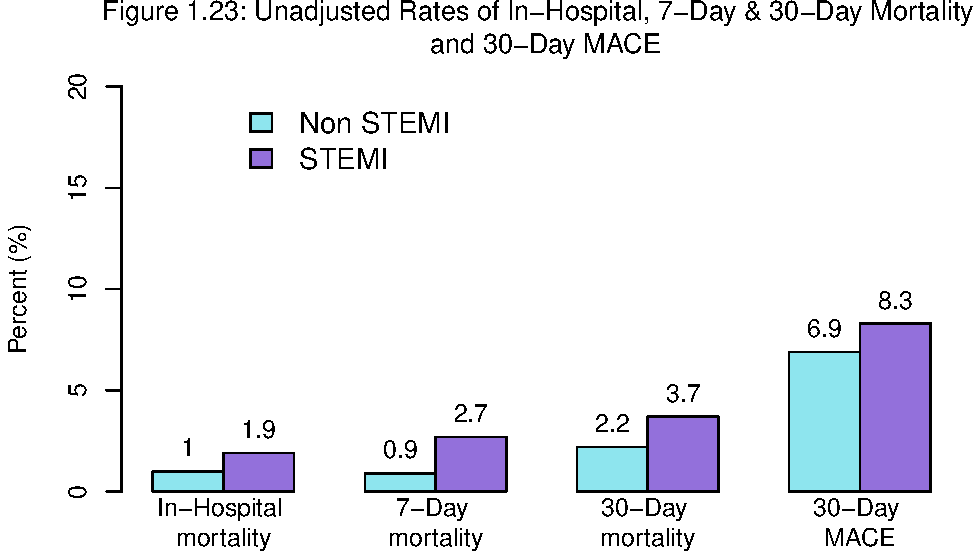
\includegraphics{ACSIS_2024_v1_pdf_files/figure-latex/unnamed-chunk-93-1.pdf}

\pagebreak

After adjustment for age and other risk factors, 7-day mortality rates
were significantly higher for patients with STEMI compared to those with
non STEMI.

~

\begin{ThreePartTable}
\begin{TableNotes}
\item[1] Adjusted for age, gender, past ACS, diabetes, hypertension, killip class $\ge$ 2, any angiography
\item[2] Definition includes: recurrent MI, recurrent ischemia, stent thrombosis, ischemic stroke, urgent
revascularization (follow-up) or death occurring within 30 days from hospitalization
\end{TableNotes}
\begin{longtable}[t]{>{\raggedright\arraybackslash}p{6.5cm}>{\centering\arraybackslash}p{4cm}>{\centering\arraybackslash}p{4cm}}
\caption{\label{tab:unnamed-chunk-95}Table 1.31: Mortality Rates by Discharge Diagnosis Adjusted for Age and Other Risk Factors}\\
\toprule
\multicolumn{1}{c}{ } & \multicolumn{2}{c}{\makecell[c]{Odds Ratio (OR) (STEMI vs. Non STEMI)\\ with 95\% Confidence Intervals (CI)}} \\
\cmidrule(l{3pt}r{3pt}){2-3}
  & Age adjusted & Risk factors adjusted\textsuperscript{1}\\
\midrule
\cellcolor{gray!10}{In-Hospital} & \cellcolor{gray!10}{2 (0.86,4.66)} & \cellcolor{gray!10}{3.36 (0.76,17.94)}\\
7-Days & 3.27 (1.25,9.53) & 7.02 (1.41,54.88)\\
\cellcolor{gray!10}{30-Days} & \cellcolor{gray!10}{1.96 (0.94,4.16)} & \cellcolor{gray!10}{4.74 (1.54,16.7)}\\
MACE\textsuperscript{2} & 1.31 (0.82,2.08) & 1.41 (0.79,2.51)\\
\bottomrule
\insertTableNotes
\end{longtable}
\end{ThreePartTable}

\pagebreak

\subsubsection{1.14.2 Rates of Mortality and MACE by
Gender}\label{rates-of-mortality-and-mace-by-gender}

~

\begin{ThreePartTable}
\begin{TableNotes}
\item[1] Definition includes: recurrent MI, recurrent ischemia, stent thrombosis, ischemic stroke, urgent
revascularization (follow-up), UAP or death occurring within 30 days from hospitalization
\end{TableNotes}
\begin{longtable}[t]{>{\raggedright\arraybackslash}p{5cm}>{\centering\arraybackslash}p{2.5cm}>{\centering\arraybackslash}p{2.5cm}>{\centering\arraybackslash}p{2.5cm}>{\centering\arraybackslash}p{2cm}}
\caption{\label{tab:unnamed-chunk-97}Table 1.32: Unadjusted Rates of In-Hospital Mortality, 7-Day Mortality, 30-Day Mortality and 30-Day MACE, by Gender}\\
\toprule
  & Total & Women & Men & p-value\\
\midrule
\cellcolor{gray!10}{n} & \cellcolor{gray!10}{1801} & \cellcolor{gray!10}{339} & \cellcolor{gray!10}{1461} & \cellcolor{gray!10}{}\\
In-hospital mortality ($\%$) & 23 (1.3) & 5 ( 1.5) & 18 (1.3) & 0.944\\
\cellcolor{gray!10}{7-day mortality ($\%$)} & \cellcolor{gray!10}{18 (1.6)} & \cellcolor{gray!10}{4 ( 1.9)} & \cellcolor{gray!10}{14 (1.5)} & \cellcolor{gray!10}{0.971}\\
30-day mortality ($\%$) & 30 (2.8) & 6 ( 3.0) & 24 (2.8) & 1.000\\
\cellcolor{gray!10}{MACE\textsuperscript{1} ($\%$)} & \cellcolor{gray!10}{81 (7.5)} & \cellcolor{gray!10}{24 (11.7)} & \cellcolor{gray!10}{57 (6.5)} & \cellcolor{gray!10}{0.018}\\
\bottomrule
\insertTableNotes
\end{longtable}
\end{ThreePartTable}

~

~

~

\begin{ThreePartTable}
\begin{TableNotes}
\item[1] Adjusted for age, past ACS, diabetes, hypertension, killip class $\geq$ 2, any angiography
\item[2] Definition includes: recurrent MI, recurrent ischemia, stent thrombosis, ischemic stroke, urgent revascularization (follow-up), UAP or death occurring within 30 days from hospitalization.
\end{TableNotes}
\begin{longtable}[t]{>{\raggedright\arraybackslash}p{6.5cm}>{\centering\arraybackslash}p{4.3cm}>{\centering\arraybackslash}p{4.3cm}}
\caption{\label{tab:unnamed-chunk-98}Table 1.33: Odds Ratios for Mortality and MACE by Gender Adjusted for Age and Other Risk Factors}\\
\toprule
\multicolumn{1}{c}{} & \multicolumn{2}{c}{OR (Women vs. Men) with 95\% CI} \\
\cmidrule(l{3pt}r{3pt}){2-3}
  & Age Adjusted & Risk factors Adjusted\textsuperscript{1}\\
\midrule
\cellcolor{gray!10}{In-Hospital mortality} & \cellcolor{gray!10}{1.05 (0.34,2.73)} & \cellcolor{gray!10}{1.13 (0.15,5.55)}\\
7-Days mortality & 1.22 (0.34,3.57) & 1.35 (0.18,6.63)\\
\cellcolor{gray!10}{30-Days mortality} & \cellcolor{gray!10}{0.89 (0.32,2.12)} & \cellcolor{gray!10}{0.4 (0.06,1.63)}\\
MACE\textsuperscript{2} & 1.7 (1,2.84) & 1.62 (0.84,3.03)\\
\bottomrule
\insertTableNotes
\end{longtable}
\end{ThreePartTable}

\pagebreak

\subsection{1.15 Re-Hospitalization within 90 Days of
Admission}\label{re-hospitalization-within-90-days-of-admission}

Re-hospitalization rates for patients with STEMI and non STEMI were
similar. Differences in reasons for re-hospitalization were not
statistically significant.

~

\begin{ThreePartTable}
\begin{TableNotes}
\item[1] Re-hospitalization among hospital survivors
\end{TableNotes}
\begin{longtable}[t]{>{\raggedright\arraybackslash}p{5cm}>{\centering\arraybackslash}p{2.5cm}>{\centering\arraybackslash}p{2.5cm}>{\centering\arraybackslash}p{2.5cm}>{\centering\arraybackslash}p{2cm}}
\caption{\label{tab:unnamed-chunk-100}Table 1.34: Re-Hospitalization within 90 Days of Admission}\\
\toprule
  & Total & Non STEMI & STEMI & p-value\\
\midrule
\addlinespace[0.3em]
\multicolumn{5}{l}{\textbf{All patients}}\\
\hspace{1em}\cellcolor{gray!10}{n} & \cellcolor{gray!10}{1720} & \cellcolor{gray!10}{1084} & \cellcolor{gray!10}{636} & \cellcolor{gray!10}{}\\
\hspace{1em}Re-hospitalization\textsuperscript{1} ($\%$) & 284 (27.6) & 174 (28.0) & 110 (26.9) & 0.746\\
\addlinespace[0.3em]
\multicolumn{5}{l}{\textbf{Re-hospitalized patients only}}\\
\hspace{1em}\cellcolor{gray!10}{n} & \cellcolor{gray!10}{285} & \cellcolor{gray!10}{175} & \cellcolor{gray!10}{110} & \cellcolor{gray!10}{}\\
\hspace{1em}Scheduled ($\%$) & 128 (46.2) & 79 (46.2) & 49 ( 46.2) & 1.000\\
\hspace{1em}\hspace{2em}\cellcolor{gray!10}{Scheduled due to cardiac reason ($\%$)} & \cellcolor{gray!10}{123 (96.9)} & \cellcolor{gray!10}{75 (94.9)} & \cellcolor{gray!10}{48 (100.0)} & \cellcolor{gray!10}{0.289}\\
\hspace{1em}Non-Scheduled ($\%$) & 149 (53.8) & 92 (53.8) & 57 ( 53.8) & 1.000\\
\hspace{1em}\hspace{2em}\cellcolor{gray!10}{Non-Scheduled due to cardiac reason ($\%$)} & \cellcolor{gray!10}{81 (54.4)} & \cellcolor{gray!10}{56 (60.9)} & \cellcolor{gray!10}{25 ( 43.9)} & \cellcolor{gray!10}{0.063}\\
\bottomrule
\insertTableNotes
\end{longtable}
\end{ThreePartTable}

\pagebreak

\subsection{1.16 Detailed 90-Day Follow-Up Clinical
Data}\label{detailed-90-day-follow-up-clinical-data}

This is the first time we performed 90 days follow up survey. We
performed this survey in order to evaluate patient's adherence to
treatment and life-style changes recommendations.

Ninety-day follow-up was performed for 1047 (58\%) patients. Of which
605 (58\%) were contacted by phone, 84 (8\%) by clinical visits and NA
(NA\%) by virtual communication. Most of the patients were asymptomatic
and in NYHA Class I.

Very few patients were treated with angiotensin receptor-neprilysin
inhibitors (ARNI'S) or SGLT-2i (non-diabetic). Most of the patients were
receiving potent statins and only 1\% were on PCSK-9i. For diabetic
patients, 35\% of patients were receiving SGLT-2 but very few patients
were on GLP1-RA.

~

\begin{ThreePartTable}
\begin{TableNotes}
\item[1] Statins include: Simvastatin, Pravastatin, Atorvastatin, Rosuvastatin
\end{TableNotes}
\begin{longtable}[t]{>{\raggedright\arraybackslash}p{8cm}>{\centering\arraybackslash}p{6.5cm}}
\caption{\label{tab:unnamed-chunk-102}Table 1.35: Medical Treatment at 90-Day Follow-Up}\\
\toprule
  & Overall\\
\midrule
\cellcolor{gray!10}{n} & \cellcolor{gray!10}{1047}\\
Aspirin ($\%$) & 782 ( 78.5)\\
\cellcolor{gray!10}{Clopidogrel ($\%$)} & \cellcolor{gray!10}{243 ( 24.4)}\\
Prasugrel ($\%$) & 348 ( 34.9)\\
\cellcolor{gray!10}{Ticagrelor ($\%$)} & \cellcolor{gray!10}{215 ( 21.6)}\\
Apixaban ($\%$) & 73 (  7.3)\\
\cellcolor{gray!10}{Dabigatran ($\%$)} & \cellcolor{gray!10}{996 (100.0)}\\
Rivaroxaban ($\%$) & 6 (  0.6)\\
\cellcolor{gray!10}{Warfarin ($\%$)} & \cellcolor{gray!10}{6 (  0.6)}\\
Enoxaparin ($\%$) & 11 (  1.1)\\
\cellcolor{gray!10}{ACE-I ($\%$)} & \cellcolor{gray!10}{429 ( 43.1)}\\
ARB's ($\%$) & 218 ( 21.9)\\
\cellcolor{gray!10}{ARNI ($\%$)} & \cellcolor{gray!10}{28 (  2.8)}\\
Spironolactone ($\%$) & 167 ( 16.8)\\
\cellcolor{gray!10}{Beta blockers ($\%$)} & \cellcolor{gray!10}{635 ( 63.8)}\\
Digoxin ($\%$) & 4 (  0.4)\\
\cellcolor{gray!10}{CCB ($\%$)} & \cellcolor{gray!10}{159 ( 16.0)}\\
Diuretics ($\%$) & 144 ( 14.5)\\
\cellcolor{gray!10}{PPI's ($\%$)} & \cellcolor{gray!10}{618 ( 62.0)}\\
Dapagliflozin (Forxiga) for non diabetic ($\%$) & 32 (  5.5)\\
\cellcolor{gray!10}{Empagliflozin (Jardiance) for non diabetic ($\%$)} & \cellcolor{gray!10}{31 (  5.4)}\\
\bottomrule
\insertTableNotes
\end{longtable}
\end{ThreePartTable}

\begin{table}[H]
\centering
\caption{\label{tab:unnamed-chunk-104}Table 1.36: Diabetes Medications in 90-Day Follow-Up}
\centering
\begin{tabular}[t]{>{\raggedright\arraybackslash}p{8cm}>{\centering\arraybackslash}p{6.5cm}}
\toprule
  & Overall\\
\midrule
\cellcolor{gray!10}{n} & \cellcolor{gray!10}{754}\\
Insulin SC (\%) & 103 ( 24.6)\\
\cellcolor{gray!10}{Glibenclamide (Gluben) (\%)} & \cellcolor{gray!10}{418 (100.0)}\\
Glipizide (Gluco-Rite) (\%) & 418 (100.0)\\
\cellcolor{gray!10}{Glimepiride (Amaryl) (\%)} & \cellcolor{gray!10}{2 (  0.5)}\\
\addlinespace
Metformin (Glucophage) (\%) & 121 ( 28.9)\\
\cellcolor{gray!10}{Sitagliptine (Januvia) (\%)} & \cellcolor{gray!10}{13 (  3.1)}\\
Saxagliptine (Onglyza) (\%) & 418 (100.0)\\
\cellcolor{gray!10}{Vidagliptine (Galvus) (\%)} & \cellcolor{gray!10}{3 (  0.7)}\\
Linagliptine (Trajenta) (\%) & 5 (  1.2)\\
\addlinespace
\cellcolor{gray!10}{Exenatide (Byetta, Budyreon) (\%)} & \cellcolor{gray!10}{418 (100.0)}\\
Liraglutide (Victoza) (\%) & 5 (  1.2)\\
\cellcolor{gray!10}{Dulaglutide (Trulicity) (\%)} & \cellcolor{gray!10}{26 (  6.2)}\\
Semaglutide (Ozempic) (\%) & 24 (  5.7)\\
\cellcolor{gray!10}{Dapagliflozin (Forxiga) (\%)} & \cellcolor{gray!10}{50 ( 12.0)}\\
\addlinespace
Empagliflozin (Jardiance) (\%) & 97 ( 23.2)\\
\cellcolor{gray!10}{Acrabose (Prandase) (\%)} & \cellcolor{gray!10}{418 (100.0)}\\
Meglinitides (Repaglinide, Novonorm) (\%) & 2 (  0.5)\\
\cellcolor{gray!10}{TZDs (Pioglitasone - actos, Rosiglitazone - Avandia) (\%)} & \cellcolor{gray!10}{3 (  0.7)}\\
\bottomrule
\end{tabular}
\end{table}

~

Concerning life-style modification, 24\% of patients reported to perform
regular weekly exercise and 41\% patients reported about diet change.
Smoking cessation was reported in 159 (40\%) of the patients who were
active smokers during the index hospitalization.

Despite the recommendation for cardiac rehabilitation programs, only
40\% of patients were actively participating or scheduled. \pagebreak

--\textgreater{}

--\textgreater{}

--\textgreater{}

--\textgreater{}

--\textgreater{}

--\textgreater{}

--\textgreater{}

--\textgreater{}

--\textgreater{}

--\textgreater{}

--\textgreater{}

--\textgreater{}

\end{document}
